\documentclass[12pt,a4paper]{report}

% ---------------- Packages ----------------
\usepackage[utf8]{inputenc}
\usepackage[T1]{fontenc}
\usepackage{xcolor}
\usepackage{graphicx}
\usepackage{geometry}
\usepackage{setspace}
\usepackage{enumitem}
\usepackage{needspace}
\usepackage{titlesec}
\usepackage{fancyhdr}
\usepackage{listings}
\usepackage{booktabs}
\usepackage{longtable}
\usepackage{array}
\usepackage{float}
\usepackage{url}
\usepackage{tikz}
\usetikzlibrary{shapes.geometric,arrows.meta,positioning,calc}
\usepackage[hidelinks]{hyperref}

% =====================================================
%  PROJECT DETAILS  (edit these in ONE place)
% =====================================================
\newcommand{\ProjectTitle}{Multi-Branch Restaurant Ordering and Management System -- Beef With Chef Melbin}
\newcommand{\ProjectTitleCaps}{MULTI-BRANCH RESTAURANT ORDERING AND MANAGEMENT SYSTEM -- BEEF WITH CHEF MELBIN}
\newcommand{\ProjectShort}{Beef With Chef Melbin}
\newcommand{\SubmissionDate}{NOVEMBER 2026}

\newcommand{\GuideName}{Ms.~Vidya N}
\newcommand{\GuideDesig}{Assistant Professor}
\newcommand{\CoordinatorName}{Ms.~Ankitha Philip}
\newcommand{\HODName}{Dr.~Rani~Saritha~R.}

% Team members: name and register number
\newcommand{\MemberOne}{MELBIN PAUL - MGP25MCA-2046}
\newcommand{\MemberTwo}{AIVIN JINU - MGP25MCA-2008}
\newcommand{\MemberThree}{AMINA SALIM - MGP25MCA-2015}
\newcommand{\MemberFour}{NANDANA RAJENDRAN - MGP25MCA-2050}

% ---------------- Page Setup ----------------
\geometry{left=1in,right=1in,top=1in,bottom=1in}
\onehalfspacing
\setlength{\parindent}{0pt}
\setlength{\parskip}{8pt}
\setlength{\headheight}{14pt}
\setlist{topsep=2pt,itemsep=3pt,parsep=0pt}

% ---------------- Custom Font Commands ----------------
\newcommand{\headingSixteen}[1]{{\fontsize{16pt}{18pt}\selectfont\textbf{#1}}}
\newcommand{\headingFourteen}[1]{{\fontsize{14pt}{16pt}\selectfont\textbf{#1}}}

% ---------------- Section Formatting ----------------
\titlespacing*{\section}{0pt}{14pt}{10pt}
\titlespacing*{\subsection}{0pt}{12pt}{8pt}
\titleformat{\section}
  {\bfseries\fontsize{14pt}{16pt}\selectfont}{\thesection}{1em}{}
\titleformat{\subsection}
  {\bfseries\fontsize{12pt}{14pt}\selectfont}{\thesubsection}{1em}{}

% Numbered chapters: CHAPTER n / TITLE centred on its own page
\titleformat{\chapter}[display]
  {\centering\fontsize{16pt}{18pt}\selectfont\bfseries}
  {\vspace*{\fill}CHAPTER \thechapter}{10pt}
  {\MakeUppercase}
  [\vspace*{\fill}\clearpage]
\titlespacing*{\chapter}{0pt}{0pt}{0pt}

% ---------------- Header & Footer ----------------
\fancypagestyle{maincontent}{
  \fancyhf{}
  \fancyhead[R]{\small \textit{\ProjectShort{} -- Multi-Branch Restaurant Management System}}
  \fancyfoot[L]{\small \textit{Saintgits College of Engineering (Autonomous)}}
  \fancyfoot[R]{\small \thepage}
  \renewcommand{\headrulewidth}{0pt}
  \renewcommand{\footrulewidth}{0pt}
}
% Chapter title pages: no header, no footer
\fancypagestyle{plain}{
  \fancyhf{}
  \renewcommand{\headrulewidth}{0pt}
  \renewcommand{\footrulewidth}{0pt}
}

% ---------------- Table of Contents rows ----------------
\newcommand{\chrow}[3]{\textbf{CHAPTER #1} & \textbf{\MakeUppercase{#2}} & \textbf{\pageref{#3}}\\[3pt]}
\newcommand{\secrow}[3]{#1 & #2 & \pageref{#3}\\}

% ---------------- Code listings ----------------
\lstdefinelanguage{JavaCustom}{
  keywords={abstract,assert,boolean,break,byte,case,catch,char,class,const,continue,default,do,double,else,enum,extends,final,finally,float,for,goto,if,implements,import,instanceof,int,interface,long,native,new,package,private,protected,public,return,short,static,strictfp,super,switch,synchronized,this,throw,throws,transient,try,void,volatile,while,true,false,null},
  sensitive=true,
  morecomment=[l]{//},
  morecomment=[s]{/*}{*/},
  morestring=[b]',
  morestring=[b]"
}
\lstset{
  language=JavaCustom,
  basicstyle=\ttfamily\footnotesize,
  frame=single,
  rulecolor=\color{black!30},
  numbers=none,
  columns=flexible,
  keepspaces=true,
  breaklines=true,
  showstringspaces=false,
  xleftmargin=0pt,
  aboveskip=8pt,
  belowskip=8pt
}

% ---------------- Image helper ----------------
\newcommand{\figimg}[3]{%
  \IfFileExists{#2}{\includegraphics[width=#1]{#2}}{%
    \fbox{\parbox[c][5cm][c]{#1}{\centering\textit{[#3]}\\ \footnotesize (add file: \detokenize{#2})}}}}

% ---------------- Schema table helpers ----------------
\newcommand{\schemahead}{\hline \textbf{Field} & \textbf{Data Type} & \textbf{Constraints} & \textbf{Description} \\ \hline}

% ---------------- TikZ styles ----------------
\tikzset{
  box/.style={draw, rounded corners=3pt, align=center, minimum height=1cm,
              minimum width=3.4cm, fill=blue!7, font=\small},
  ent/.style={draw, align=center, minimum height=1cm, minimum width=3cm,
              fill=blue!7, font=\small\bfseries},
  proc/.style={draw, rounded corners=3pt, align=center, minimum height=0.8cm,
               minimum width=5.6cm, fill=blue!7, font=\small, text width=5.4cm},
  dec/.style={draw, diamond, aspect=3, align=center, fill=yellow!15,
              font=\footnotesize, inner sep=1pt, text width=3.6cm},
  term/.style={draw, rounded corners=8pt, align=center, fill=green!12,
               minimum height=0.7cm, minimum width=2.4cm, font=\small},
  rej/.style={draw, rounded corners=3pt, align=center, fill=red!10,
              minimum height=0.8cm, font=\small, text width=2.6cm},
  arr/.style={-{Stealth[length=2.2mm]}, thick},
  lab/.style={font=\scriptsize, fill=white, inner sep=1pt}
}

\begin{document}

% =====================================================
% PAGE 1 : TITLE PAGE
% =====================================================
\thispagestyle{empty}
\enlargethispage{1.2cm}

\begin{center}

\vspace*{0.2cm}

\headingSixteen{CAPSTONE PROJECT PRELIMINARY REPORT}\\[0.2cm]

\headingFourteen{ON}\\[0.2cm]

\headingSixteen{\textcolor{blue}{\ProjectTitleCaps}}\\[0.5cm]

\headingFourteen{Submitted By}\\[0.12cm]

\headingFourteen{\textcolor{blue}{\MemberTwo}}\\[0.45cm]

\headingFourteen{\textcolor{blue}{\MemberThree}}\\[0.45cm]

\headingFourteen{\textcolor{blue}{\MemberOne}}\\[0.45cm]

\headingFourteen{\textcolor{blue}{\MemberFour}}\\[0.45cm]

\headingFourteen{To}\\[0.12cm]

\textit{the APJ Abdul Kalam Technological University in partial}\\
\textit{fulfillment of the requirements for the award of the degree of}\\[0.3cm]

\headingFourteen{MASTER OF COMPUTER APPLICATIONS}\\[0.5cm]

\headingFourteen{Under the guidance of}\\[0.15cm]

\headingFourteen{\textcolor{blue}{\GuideName}}\\[0.1cm]
\headingFourteen{\textcolor{blue}{\GuideDesig}}\\[0.6cm]

\figimg{3.5cm}{Saintgits logo New.png}{Saintgits College Logo}\\[0.4cm]

\headingFourteen{DEPARTMENT OF COMPUTER APPLICATIONS}\\[0.12cm]

\headingFourteen{SAINTGITS COLLEGE OF ENGINEERING (AUTONOMOUS)}\\

\headingFourteen{Pathamuttom, Kottayam, Kerala -- 686532}\\[0.35cm]

\textit{(Approved by AICTE and affiliated to APJ Abdul Kalam Technological University)}
\\[0.6cm]

\headingSixteen{\SubmissionDate}

\end{center}

% =====================================================
% PAGE 2 : BONAFIDE CERTIFICATE
% =====================================================
\newpage
\thispagestyle{empty}

\begin{center}

\fontsize{16pt}{18pt}\selectfont
\textbf{SAINTGITS COLLEGE OF ENGINEERING (AUTONOMOUS)}\\

Kottukulam Hills, Pathamuttom, Kottayam, Kerala -- 686532

\end{center}

\vspace{0.2cm}

\begin{center}
\figimg{4.5cm}{Saintgits logo New.png}{Saintgits College Logo}
\end{center}

\vspace{0.1cm}

\begin{center}

\fontsize{16pt}{18pt}\selectfont
\textbf{BONAFIDE CERTIFICATE}

\end{center}

\vspace{0.2cm}

Certified that the report entitled \textbf{“\ProjectTitle{}”} submitted by
\textbf{“\MemberTwo”}, \textbf{“\MemberThree”},
\textbf{“\MemberOne”}, \textbf{“\MemberFour”} to the APJ
Abdul Kalam Technological University in partial fulfillment of the requirements for the award of the
Degree of \textbf{Master of Computer Applications} is a bonafide record of the project work carried
out by them under our guidance and supervision. This report in any form has not been submitted
to any other University or Institute for any purpose.

\vspace{2cm}

% =====================================================
% SIGNATURE SECTION
% =====================================================
\begin{center}
\begin{tabular}{@{}p{0.50\textwidth}@{\hspace{0.02\textwidth}}p{0.40\textwidth}@{}}
\raggedright
\textbf{\GuideName}\\
Internal Guide
&
\raggedleft
\textbf{\CoordinatorName}\\
Project Coordinator
\end{tabular}
\end{center}

\vspace{2.5cm}

% =====================================================
% HEAD OF DEPARTMENT
% =====================================================
\begin{center}
\textbf{\HODName}\\
Head of the Department
\end{center}

% ===================== PAGE 3 : ACKNOWLEDGEMENT =====================
\newpage
\thispagestyle{empty}

\begin{center}
\fontsize{16pt}{18pt}\selectfont
\textbf{ACKNOWLEDGEMENT}
\end{center}

\vspace{1cm}

At the outset, we thank the Lord Almighty for His abundant grace, strength and hope to make our
endeavour a success. We express our deep-felt gratitude to \textbf{Dr.~Sudha~T.}, Principal,
Saintgits College of Engineering (Autonomous), for her warm support with regard to the work and
to the management for providing the facilities required.

We would like to place our deep sense of gratitude to
\textbf{Prof.~Mini~Punnoose}, Director MCA, Saintgits College of Engineering
(Autonomous), for her constant encouragement. We express our gratitude to
\textbf{\HODName}, Head of the Department, Department of Computer
Applications, Saintgits College of Engineering (Autonomous), for her support
and guidance.

We are profoundly grateful to \textbf{\GuideName}, our Project Guide and
\textbf{\CoordinatorName}, the Project Coordinator, for their valuable guidance, help,
suggestions and assessment throughout the course of this work.

Furthermore, we would like to thank all others, especially our parents and numerous friends.
This project report would not have been a success without their inspiration, valuable
suggestions and moral support from them throughout its course.

\vspace{2cm}

\begin{flushright}
\textbf{Aivin Jinu}\\
\textbf{Amina Salim}\\
\textbf{Melbin Paul}\\
\textbf{Nandana Rajendran}
\end{flushright}

% ===================== PAGE 4 : SIMILARITY REPORT =====================
\newpage
\thispagestyle{empty}

\begin{center}
    \fontsize{16pt}{18pt}\selectfont
    \textbf{SIMILARITY REPORT}
\end{center}

\vspace{1cm}

This is to certify that the Capstone Project Report entitled \textbf{“\ProjectTitle{}”} has been analyzed using institutional plagiarism detection software.

\vspace{0.8cm}

\begin{center}
\begin{tabular}{|p{4.5cm}|p{9.5cm}|}
\hline
\textbf{Parameter} & \textbf{Details} \\ \hline
\textbf{Title of Report} & \ProjectTitle{} \\ \hline
\textbf{Authors} & Melbin Paul, Aivin Jinu, Amina Salim, Nandana Rajendran \\ \hline
\textbf{Program} & Master of Computer Applications (MCA) \\ \hline
\textbf{Institution} & Saintgits College of Engineering (Autonomous) \\ \hline
\textbf{Affiliation} & APJ Abdul Kalam Technological University \\ \hline
\textbf{Similarity Index} & Verified within prescribed institutional threshold ($< 10\%$) \\ \hline
\textbf{Status} & Certified Original Technical Work \\ \hline
\end{tabular}
\end{center}

\vspace{1cm}

The contents of this report represent original project development and scholarly documentation carried out by the team members under the guidance of the Department of Computer Applications.

% ===================== PAGE 5 : ABSTRACT =====================
\newpage
\thispagestyle{empty}

\begin{center}
\fontsize{16pt}{18pt}\selectfont
\textbf{ABSTRACT}
\end{center}

\vspace{1cm}

The Multi-Branch Restaurant Ordering and Management System -- Beef With Chef Melbin is a comprehensive, production-grade enterprise software platform designed to unify online food ordering, dining-room table management, and back-of-house kitchen and delivery logistics across multi-location restaurant chains. Modern hospitality enterprises face severe operational fragmentation when relying on disparate standalone point-of-sale terminals, third-party delivery aggregators with exorbitant commissions, manual paper registers, and uncoordinated kitchen messaging. Beef With Chef Melbin addresses these bottlenecks through a centralized, multi-tenant architectural design built on Angular 21, Java 21, Spring Boot 4.0.7, and MySQL 8.0.\par

The platform integrates four distinct operational workflows tailored to specific user roles: Super Administrators and Branch Managers, Kitchen Chefs, Floor \& Delivery Employees, and Customers. At the dining premises, guests utilize dynamic QR-code table ordering, where scanning a table-affixed code automatically binds the order session to the specific restaurant table and branch, eliminating order-taking wait times. For doorstep delivery, the backend enforces automated geospatial validation using the mathematical Haversine formula, restricting delivery requests strictly to within a 10.0-kilometer radius of the selected branch. The kitchen operates via a dedicated Kitchen Display System (KDS) with sound-alert notifications, enabling chefs to transition orders seamlessly through live preparation stages (Placed, Preparing, Ready). Floor staff and delivery personnel utilize an employee console to claim available deliveries, update progress stages (Accepted, Picked Up, Out for Delivery, Delivered), and service dine-in guests.\par

The system further incorporates real-time raw material inventory tracking with automated low-stock warnings, table reservations, multiple payment methods (Card, UPI, Cash, Wallet, Net Banking, and Demo simulation), customer blacklisting for fraud mitigation, website media content management, and centralized business intelligence analytics. Strict branch isolation is enforced via custom security utilities, ensuring branch personnel only access data pertinent to their location while granting administrators global visibility. By replacing manual workflows with an automated, synchronized, and resilient digital infrastructure, the system substantially enhances order accuracy, reduces customer wait times, optimizes delivery efficiency, and empowers restaurant management with real-time actionable insights.

% ===================== TABLE OF CONTENTS =====================
\newpage
\thispagestyle{empty}
\begin{center}
\headingFourteen{TABLE OF CONTENTS}
\end{center}
\vspace{0.15cm}
{\singlespacing
\small
\renewcommand{\arraystretch}{1.05}
\setlength{\parskip}{0pt}
\begin{longtable}{@{}p{3cm}p{9cm}>{\centering\arraybackslash}p{1.9cm}@{}}
\textbf{CHAPTER} & \multicolumn{1}{>{\centering\arraybackslash}p{9cm}}{\textbf{TITLE}} & \multicolumn{1}{>{\centering\arraybackslash}p{1.9cm}}{\textbf{PAGE NO.}}\\[6pt]
\endfirsthead
\textbf{CHAPTER NO.} & \multicolumn{1}{>{\centering\arraybackslash}p{9cm}}{\textbf{TITLE}} & \multicolumn{1}{>{\centering\arraybackslash}p{1.9cm}}{\textbf{PAGE NO.}}\\[6pt]
\endhead
\chrow{1}{Introduction}{ch1}
\secrow{1.1}{Project Overview}{s11}
\secrow{1.2}{Objectives of the Project}{s12}
\secrow{1.3}{Scope and Availability}{s13}
\chrow{2}{Requirement Analysis}{ch2}
\secrow{2.1}{Existing System / Problem Statement}{s21}
\secrow{2.2}{Proposed System / Solution Overview}{s22}
\secrow{2.3}{Feasibility Study}{s23}
\secrow{2.4}{Conceptual Modeling}{s24}
\secrow{2.5}{Planning and Scheduling}{s25}
\chrow{3}{System Specification}{ch3}
\secrow{3.1}{Software and Hardware Requirements}{s31}
\secrow{3.1.1}{Software Requirements}{s311}
\secrow{3.1.2}{Hardware Requirements}{s312}
\secrow{3.2}{Functional Specifications}{s32}
\secrow{3.3}{Tools and Platforms Used}{s33}
\secrow{3.4}{Development Environment}{s34}
\chrow{4}{System Design}{ch4}
\secrow{4.1}{Module Description}{s41}
\secrow{4.2}{Data / Schema Design}{s42}
\secrow{4.3}{Procedural / Flow Design}{s43}
\secrow{4.4}{User Interface Design}{s44}
\chrow{5}{Development Methodology}{ch5}
\secrow{5.1}{Project Roadmap}{s51}
\secrow{5.2}{User Stories}{s52}
\secrow{5.3}{Test Plan}{s53}
\chrow{6}{Implementation and Testing}{ch6}
\secrow{6.1}{Implementation Procedures}{s61}
\secrow{6.2}{Testing Methods and Results}{s62}
\chrow{7}{Conclusion and Future Scope}{ch7}
\secrow{7.1}{Limitations}{s71}
\secrow{7.2}{Future Scope}{s72}
\secrow{7.3}{Conclusion}{s73}
\chrow{8}{Appendix}{ch8}
\secrow{8.1}{Sample Code / Queries}{s81}
\secrow{8.2}{Screenshots}{s82}
\secrow{8.3}{Git Logs}{s83}
\chrow{9}{References}{ch9}
\secrow{9.1}{References}{s91}
\end{longtable}
}

% ===================== LIST OF ABBREVIATIONS =====================
\newpage
\thispagestyle{empty}
\begin{center}
\headingFourteen{List of Abbreviations}
\end{center}
\vspace{0.7cm}
{\singlespacing
\small
\renewcommand{\arraystretch}{1.45}
\setlength{\parskip}{0pt}
\begin{longtable}{@{}p{2.7cm}p{11cm}@{}}
\textbf{API:} & Application Programming Interface\\
\textbf{CI/CD:} & Continuous Integration and Continuous Deployment\\
\textbf{CORS:} & Cross-Origin Resource Sharing\\
\textbf{CRUD:} & Create, Read, Update, Delete\\
\textbf{CSS:} & Cascading Style Sheets\\
\textbf{DTO:} & Data Transfer Object\\
\textbf{ERD:} & Entity Relationship Diagram\\
\textbf{GPS:} & Global Positioning System\\
\textbf{HTML:} & HyperText Markup Language\\
\textbf{HTTP:} & HyperText Transfer Protocol\\
\textbf{IDE:} & Integrated Development Environment\\
\textbf{JPA:} & Java Persistence API\\
\textbf{JSON:} & JavaScript Object Notation\\
\textbf{JWT:} & JSON Web Token\\
\textbf{KDS:} & Kitchen Display System\\
\textbf{ORM:} & Object-Relational Mapping\\
\textbf{POJO:} & Plain Old Java Object\\
\textbf{POS:} & Point of Sale\\
\textbf{QR:} & Quick Response\\
\textbf{RAM:} & Random Access Memory\\
\textbf{REST:} & Representational State Transfer\\
\textbf{SDK:} & Software Development Kit\\
\textbf{SPA:} & Single Page Application\\
\textbf{SQL:} & Structured Query Language\\
\textbf{UI:} & User Interface\\
\textbf{URI:} & Uniform Resource Identifier\\
\textbf{URL:} & Uniform Resource Locator\\
\textbf{UX:} & User Experience\\
\end{longtable}
}

\newpage
\pagenumbering{arabic}
\pagestyle{maincontent}

% =====================================================
%                     CHAPTER 1
% =====================================================
\chapter{Introduction}\label{ch1}

\section{Project Overview}\label{s11}
The hospitality and food service industry is experiencing a profound technological transformation driven by rising customer expectations for digital convenience, contactless interactions, and rapid order fulfillment. Multi-location restaurant chains face formidable operational challenges in maintaining consistency across branch operations, balancing in-house dining with high-volume delivery logistics, and tracking ingredient stock across multiple geographically separated kitchens.

The Multi-Branch Restaurant Ordering and Management System -- Beef With Chef Melbin is an enterprise-grade digital solution architected specifically to overcome these modern restaurant management hurdles. The platform bridges the divide between customer-facing storefronts and back-of-house kitchen and delivery workflows by uniting all restaurant activities within a single, coherent, synchronized digital ecosystem.

The system comprises two core components working in seamless synchronization: a high-performance, responsive Single Page Application (SPA) frontend developed using Angular 21, and a robust, scalable RESTful backend service built on Java 21 and Spring Boot 4.0.7, backed by a persistent MySQL 8.0 relational database. The platform caters to five distinct user roles: Super Administrators, Branch Managers, Kitchen Chefs, Floor \& Delivery Employees, and Customers.

For dining guests at physical restaurant premises, the system introduces dynamic QR-code table ordering. Each dining table is equipped with a unique QR code which, when scanned using any smartphone camera, immediately launches the restaurant ordering interface with the specific branch and table pre-assigned. This empowers customers to browse the digital menu, customize their culinary selections, place orders directly to the kitchen, and settle payments without requiring manual waiter intervention.

For doorstep delivery orders, the platform incorporates strict geospatial boundary validation implemented via the mathematical Haversine formula. The system validates customer coordinates in real time, permitting delivery orders only if the delivery address falls within a strict 10.0-kilometer radius of the servicing branch, thereby safeguarding food quality, minimizing transit delays, and avoiding logistical failure.

Behind the scenes, the Kitchen Display System (KDS) provides culinary staff with a live, real-time board of pending and preparing orders accompanied by automated audio and visual notifications. Floor employees and delivery riders interact with an employee console to claim available delivery orders, track their progress through out-for-delivery and delivered states, and coordinate dining room service. Meanwhile, Branch Managers and Administrators benefit from comprehensive oversight, including raw material inventory tracking with low-stock alerts, table reservations, customer blacklisting, and business intelligence reporting.

\section{Objectives of the Project}\label{s12}
The primary objective of the Multi-Branch Restaurant Ordering and Management System -- Beef With Chef Melbin is to design, develop, and deploy an automated, secure, and unified digital platform that optimizes restaurant operations, improves order accuracy, and elevates customer satisfaction across multiple branch locations.

The specific objectives of the project are:
\begin{enumerate}[leftmargin=*]
  \item \textbf{To automate multi-branch order processing:} Develop a unified ordering pipeline supporting Dine-In, Takeaway, and Delivery order types with real-time status transitions from placement to final fulfillment.
  \item \textbf{To enable contactless QR code dining:} Implement dynamic QR-code table ordering that enables restaurant guests to view menus, place orders, and make payments directly from their smartphones, eliminating waiter dependency and reducing table turnaround time.
  \item \textbf{To enforce geospatial delivery boundary validation:} Integrate the mathematical Haversine algorithm within the backend API to strictly enforce a 10.0-km maximum delivery radius from the branch's GPS coordinates, preventing out-of-bounds orders and logistics bottlenecks.
  \item \textbf{To streamline kitchen operations via Chef KDS:} Build an interactive Kitchen Display System (KDS) for kitchen chefs featuring audio-visual order alerts, order item breakdowns, and one-click status transitions from Placed to Preparing and Ready.
  \item \textbf{To coordinate delivery and waiter workflows:} Provide dedicated employee interfaces allowing staff to claim available delivery assignments, update dispatch milestones (Accepted, Picked Up, Out for Delivery, Delivered), and manage table service.
  \item \textbf{To automate table reservations and seating:} Create an intuitive table booking system enabling customers to reserve dining tables by date, time, party size, and branch, with real-time availability checking and automated status tracking.
  \item \textbf{To track raw material inventory and thresholds:} Implement branch-level raw ingredient inventory tracking with automated stock adjustment logging (Stock-In, Stock-Out, Usage) and instant warnings when quantities breach defined low-stock thresholds.
  \item \textbf{To implement multi-tenant security and branch isolation:} Enforce strict branch-scoped authorization barriers using Spring Security, BCrypt password hashing, and stateless JSON Web Tokens (JWT), preventing unauthorized cross-branch data tampering while giving administrators global oversight.
  \item \textbf{To deliver actionable executive business intelligence:} Construct a centralized analytical dashboard that computes live financial metrics, today's sales, pending orders, delivery queues, branch-by-branch sales breakdowns, and exportable organizational reports.
  \item \textbf{To mitigate fraud via customer blacklisting:} Provide administrative controls to flag and blacklist abusive or fraudulent customer accounts, immediately terminating active sessions and restricting subsequent order placement.
\end{enumerate}

\section{Scope and Availability}\label{s13}
The scope of the Multi-Branch Restaurant Ordering and Management System encompasses complete end-to-end digitisation of restaurant workflows across multiple independent branches operating under the 'Beef With Chef Melbin' brand. The system spans customer-facing storefronts, kitchen production terminals, employee dispatch tools, and managerial oversight suites.

The operational scope covers:
\begin{itemize}[leftmargin=*]
  \item Multi-branch administrative configuration, including branch geolocation (latitude and longitude), operating hours, address details, and active status toggling.
  \item Branch-scoped food catalog and menu categorization, supporting regular, seasonal, and promotional dishes with image URLs, descriptions, and dynamic availability toggles.
  \item Dine-in table mapping, capacity management, and automatic unique QR code assignment per physical table.
  \item Interactive delivery checkout featuring Leaflet-based GPS map location picking and automated distance computation.
  \item Customer account management, profile updates, order history tracking, and order cancellation capabilities prior to kitchen preparation.
  \item Multi-channel payment simulation accommodating Card, UPI, Net Banking, Wallet, and Cash on Delivery.
  \item Ingredient inventory auditing with transaction logs and proactive low-stock warnings.
  \item Dynamic landing page branding, hero section management, and marketing content uploads via administrative website image controllers.
\end{itemize}

The system is architected as a cross-platform, cloud-ready web application accessible from any modern web browser on desktop computers, laptops, tablets, and mobile smartphones. Because the frontend is built as a fully responsive Angular 21 Single Page Application, it requires no specialized client-side software installations---customers and staff simply open the application URL or scan table QR codes using native mobile device cameras.

The backend REST API is hosted on a high-availability cloud environment (such as Render) with continuous deployment, while data persistence is managed by a managed MySQL database instance with connection pooling. The platform operates 24 hours a day, 7 days a week, providing uninterrupted accessibility for online orders, reservations, and inventory audits. System features are strictly guarded by role-based authentication, ensuring that data is accessible only to authorized personnel according to their organizational roles and branch assignments.

% =====================================================
%                     CHAPTER 2
% =====================================================
\chapter{Requirement Analysis}\label{ch2}

\section{Existing System / Problem Statement}\label{s21}
Many contemporary multi-branch restaurant chains continue to operate using fragmented, outdated legacy systems that hinder operational scalability and impair customer satisfaction. In conventional setups, in-house dining relies on manual paper-based order taking by waitstaff, physical paper kitchen order tickets (KOT), and stand-alone electronic cash registers. For online deliveries, restaurants predominantly rely on third-party food aggregator platforms.

The existing manual and semi-digital approaches present critical vulnerabilities and operational deficiencies:
\begin{itemize}[leftmargin=*]
  \item \textbf{Exorbitant Aggregator Commissions:} Third-party food delivery aggregators levy steep commission fees (often 20\% to 35\% per order), drastically diminishing profit margins and severing direct customer relationships.
  \item \textbf{Lack of Geospatial Delivery Control:} Legacy ordering systems lack automated geospatial boundary checks, resulting in delivery orders being placed from locations far beyond realistic delivery radiuses. This leads to food getting cold in transit, severe delivery delays, customer dissatisfaction, and high cancellation rates.
  \item \textbf{Order Miscommunication and Bottlenecks:} In-house paper order tickets frequently suffer from illegible handwriting, lost slips, delayed handoffs between waitstaff and chefs, and order inaccuracies, culminating in extended table turnaround times.
  \item \textbf{Data Silos Across Branches:} Multi-branch operations run disparate point-of-sale machines that fail to synchronize sales, reservations, or inventory with central management in real time, making organization-wide reporting and inventory planning arduous.
  \item \textbf{Unmonitored Raw Material Depletion:} Inventory audits are typically conducted retrospectively via manual spreadsheets at the end of the day or week. Kitchens frequently run out of key ingredients mid-service, resulting in cancelled orders and lost revenue.
  \item \textbf{Absence of Fraud and Abuse Controls:} Traditional phone or counter ordering provides zero technical mechanisms to identify or blacklist repeat fraudulent customers who routinely reject cash-on-delivery orders upon arrival.
\end{itemize}

\section{Proposed System / Solution Overview}\label{s22}
To decisively resolve the aforementioned systemic deficiencies, the proposed Multi-Branch Restaurant Ordering and Management System -- Beef With Chef Melbin introduces a centralized, cloud-integrated platform that synchronizes dining room, kitchen, delivery, inventory, and management operations in real time.

Key architectural innovations of the proposed system include:
\begin{itemize}[leftmargin=*]
  \item \textbf{Direct Web-Based Customer Portal:} A high-performance Angular Single Page Application empowering customers to browse menus, customize dishes, place dine-in, takeaway, or delivery orders, book tables, and track fulfillment without intermediary aggregator commissions.
  \item \textbf{Contactless QR-Code Table Ordering:} Each restaurant table features a durable, distinct QR code. Customers simply scan the code with their mobile device camera, immediately opening a browser ordering session tied to that precise branch and table ID, bypassing waitstaff entirely.
  \item \textbf{Automated Haversine Delivery Radius Validation:} The backend REST API executes an automated geospatial validation against customer coordinates, enforcing a strict 10.0-km radius around the selected branch before accepting any delivery order.
  \item \textbf{Real-Time Kitchen Display System (KDS):} Kitchen chefs view incoming orders on a dedicated screen that sounds audio notifications and provides clear visual tracking through 'Placed', 'Preparing', and 'Ready' milestones.
  \item \textbf{Streamlined Employee Dispatch:} Staff and delivery riders claim available orders, transition delivery milestones, and coordinate dining service through dedicated, authenticated employee interfaces.
  \item \textbf{Real-Time Inventory and Threshold Tracking:} Every inventory adjustment is recorded with transaction audits, and items breaching their low-stock threshold trigger prominent administrative alerts.
  \item \textbf{Granular Branch-Scoped Access and Fraud Mitigation:} Branch managers are restricted to data belonging to their branch, administrators have global control, and abusive accounts can be instantly blacklisted.
\end{itemize}

\section{Feasibility Study}\label{s23}
A comprehensive feasibility study was conducted prior to system development to evaluate the technical, economic, operational, schedule, and security viability of the proposed solution.
\begin{enumerate}[leftmargin=*]
  \item \textbf{Technical Feasibility:} The project utilizes industry-proven, mature, and widely adopted open-source technologies. Angular 21 provides a robust, modern framework with reactive signals and standalone components for high-speed client-side rendering. Java 21 and Spring Boot 4.0.7 deliver an enterprise-grade backend runtime renowned for multithreading efficiency, transactional integrity, and RESTful web services. MySQL 8.0 offers ACID-compliant relational storage, foreign key constraints, and optimized indexing. Standard geometric calculations via the Haversine formula are lightweight and execute in sub-millisecond time. The technical architecture is fully feasible and scalable.
  \item \textbf{Economic Feasibility:} The system is economically sound, built entirely upon open-source frameworks, compilers, and libraries that incur zero licensing fees. Development was conducted using free, community-standard IDEs (Visual Studio Code). Cloud deployment leverages scalable tiers (such as Render for web services and cloud-hosted MySQL instances). Eliminating third-party food delivery aggregators reclaims substantial operational revenue, yielding a highly favorable return on investment.
  \item \textbf{Operational Feasibility:} The system provides tailored, intuitive interfaces for all five user roles. Customers require no training---ordering via QR codes or web browsers is self-explanatory. Chefs operate a color-coded touch-friendly KDS. Delivery staff use an uncluttered dispatch list. Branch managers and administrators receive unified dashboards. The streamlined operational workflows reduce customer friction, eliminate order miscommunication, and improve employee efficiency.
  \item \textbf{Schedule Feasibility:} The development lifecycle was organized into structured phases across requirements analysis, database modeling, REST API development, Angular SPA implementation, security integration, end-to-end testing, and deployment. The modular architecture allowed independent parallel progress across backend endpoints and frontend components, ensuring completion well within the academic semester timeframe.
  \item \textbf{Security Feasibility:} The platform enforces comprehensive security standards. All user passwords are encrypted using salted BCrypt hashing before database persistence. Session management is strictly stateless, utilizing digitally signed JSON Web Tokens (JWT) containing cryptographically signed role and user claims. Custom security filters (JwtAuthFilter, BranchSecurityUtils) validate every request, ensuring multi-tenant branch isolation and blocking blacklisted users.
\end{enumerate}

\section{Conceptual Modeling}\label{s24}
The conceptual model defines the core entities, their business attributes, and the relational associations that govern the Beef With Chef Melbin restaurant ecosystem. The architecture is centered around a multi-branch hierarchy where branches operate as autonomous fulfillment hubs while remaining unified under centralized corporate administration.

The system encompasses fourteen core entities:
\begin{itemize}[leftmargin=*]
  \item \textbf{Branch:} Represents an individual restaurant location containing geographical coordinates (latitude and longitude), contact details, address, operating hours, and active status.
  \item \textbf{User:} Stores user profiles, authentication credentials, assigned roles (ADMIN, BRANCH\_MANAGER, CHEF, EMPLOYEE, CUSTOMER), branch associations, and blacklisting status.
  \item \textbf{MenuCategory:} Groups culinary offerings within a specific branch (e.g., Starters, Main Course, Chef Specials, Beverages).
  \item \textbf{FoodItem:} Represents an individual dish belonging to a category and branch, specifying price, image URL, availability toggle, and seasonal status.
  \item \textbf{RestaurantTable:} Defines dining room tables mapped to a branch, containing table number, seating capacity, table status (AVAILABLE, OCCUPIED, RESERVED), and a unique QR code.
  \item \textbf{Reservation:} Records advance dining reservations with customer contact details, party size, reservation date, time, and status.
  \item \textbf{Order:} The central transactional entity recording order type (DINE\_IN, TAKEAWAY, DELIVERY), current status, branch, customer, assigned employee, delivery coordinates, subtotal, and total amount.
  \item \textbf{OrderItem:} Child entity of Order mapping specific food items, quantities, unit prices, and line subtotals.
  \item \textbf{Payment:} Records financial settlements for an order, capturing amount, payment method (CARD, UPI, CASH, NET\_BANKING, WALLET, DEMO), payment status (PENDING, PAID, FAILED, REFUNDED), and unique transaction ID.
  \item \textbf{InventoryCategory:} Groups raw ingredients and kitchen supplies within a branch (e.g., Meats, Produce, Dairy, Spices, Dry Goods).
  \item \textbf{InventoryItem:} Represents a raw material stock item tracking quantity on hand, unit of measure (kg, liters, units), and low-stock threshold.
  \item \textbf{InventoryTransaction:} Maintains an immutable audit trail of every stock modification (STOCK\_IN, STOCK\_OUT, USAGE) with timestamps and quantity deltas.
  \item \textbf{Notification:} Delivers role-based alerts for kitchen events, ready orders, delivery assignments, and customer updates.
  \item \textbf{WebsiteImage:} Stores marketing banners, hero images, and branding assets managed by administrators.
\end{itemize}

\section{Planning and Scheduling}\label{s25}
The project followed an Agile development lifecycle incorporating iterative sprints to guarantee quality, maintainability, and systematic delivery. Work was divided across distinct functional domains, enabling continuous integration and rigorous testing at each milestone.

\begin{longtable}{|p{1.8cm}|p{5.0cm}|p{2.2cm}|p{4.8cm}|}
\hline
\textbf{Phase} & \textbf{Activity / Focus} & \textbf{Duration} & \textbf{Deliverables / Milestones} \\ \hline
\endfirsthead
\hline
\textbf{Phase} & \textbf{Activity / Focus} & \textbf{Duration} & \textbf{Deliverables / Milestones} \\ \hline
\endhead
Phase 1 & Requirement Elicitation \& Domain Analysis & Week 1 -- 2 & Detailed requirements, user personas, feasibility study, SRS document. \\ \hline
Phase 2 & System Architecture \& Database Modeling & Week 3 -- 4 & Relational schema design, entity mapping, REST API contract specification. \\ \hline
Phase 3 & Backend Core REST API \& Security Development & Week 5 -- 7 & Spring Boot setup, JWT filter, BCrypt authentication, BranchSecurityUtils. \\ \hline
Phase 4 & Ordering, QR Logic \& Haversine Delivery Engine & Week 8 -- 10 & Order pipeline, GeoUtils distance calculation, Table QR code generation. \\ \hline
Phase 5 & Frontend Angular SPA \& Theme Implementation & Week 11 -- 13 & Responsive UI, Bootstrap 5.3.3, Poppins typography, Dark/Light theme. \\ \hline
Phase 6 & Role Dashboards (Admin, Chef KDS, Employee) & Week 14 -- 15 & Chef order queue, sound alerts, employee dispatch list, admin analytics. \\ \hline
Phase 7 & Integration, Security Auditing \& System Testing & Week 16 -- 17 & End-to-end integration, boundary tests, role access verification, bug fixes. \\ \hline
Phase 8 & Final Documentation \& Deployment Preparation & Week 18 & Docker containerization, Render deployment, final capstone report. \\ \hline
\end{longtable}

% =====================================================
%                     CHAPTER 3
% =====================================================
\chapter{System Specification}\label{ch3}

\section{Software and Hardware Requirements}\label{s31}
The Multi-Branch Restaurant Ordering and Management System -- Beef With Chef Melbin operates as a distributed web application connecting an Angular 21 Single Page Application frontend with a Java 21 / Spring Boot 4.0.7 backend and a MySQL 8.0 relational database. The hardware and software environments were chosen to guarantee high computational throughput, reliable data persistence, and cross-platform accessibility.

\subsection{Software Requirements}\label{s311}
The software stack and development dependencies required for compiling, running, and maintaining the system are specified below:
\begin{itemize}[leftmargin=*]
  \item \textbf{Operating System:} Windows 11 or Linux (Ubuntu 22.04 LTS) for development, deployment, and hosting.
  \item \textbf{Frontend Framework:} Angular 21.2.0 (Standalone Components, Signals, Reactive Forms, Router).
  \item \textbf{Client Language:} TypeScript 5.9.2 and modern ECMAScript standards.
  \item \textbf{Client Styling:} Bootstrap 5.3.3, Vanilla CSS custom design tokens, Font Awesome 6.4, Poppins font.
  \item \textbf{Runtime Environment:} Node.js v20.18.0 LTS and npm 11.11.0 for client-side package management.
  \item \textbf{Backend Framework:} Java 21 (OpenJDK / Eclipse Temurin), Spring Boot 4.0.7 (WebMVC, Data JPA, Security).
  \item \textbf{Build Tool:} Apache Maven 3.9+ for backend dependency resolution, testing, and JAR compilation.
  \item \textbf{Database Engine:} MySQL 8.0 Server with InnoDB storage engine for ACID transactional compliance.
  \item \textbf{Database Driver:} MySQL Connector/J 9.0+ for high-performance JDBC connectivity.
  \item \textbf{Authentication / Token:} JSON Web Token (JJWT 0.12.6 API, Impl, Jackson) and BCryptPasswordEncoder.
  \item \textbf{Mapping / Geolocation:} Leaflet.js for interactive map coordinate selection and mathematical Haversine calculations.
  \item \textbf{Code Editor / IDE:} Visual Studio Code and IntelliJ IDEA Community Edition.
  \item \textbf{Version Control:} Git 2.40+ and GitHub for collaborative version tracking and CI/CD triggers.
  \item \textbf{API Testing:} Postman and cURL for testing and validating REST endpoints.
\end{itemize}

\subsection{Hardware Requirements}\label{s312}
The hardware specifications necessary for development, production hosting, and end-user access are detailed below:
\begin{itemize}[leftmargin=*]
  \item \textbf{Development Machine:} Intel Core i5 / AMD Ryzen 5 processor (quad-core or higher, 2.5 GHz+).
  \item \textbf{Development RAM:} 16 GB DDR4/DDR5 RAM recommended (minimum 8 GB) for concurrent Angular \& Spring Boot execution.
  \item \textbf{Local Storage:} 256 GB NVMe Solid State Drive (SSD) with at least 20 GB free space for project artifacts and dependencies.
  \item \textbf{Production Server:} Cloud VM / Container (e.g., Render Web Service) with minimum 1 vCPU, 2 GB RAM, and high-speed network bandwidth.
  \item \textbf{Database Storage:} Cloud-hosted MySQL instance with 10 GB persistent SSD storage and automated daily backups.
  \item \textbf{Client Smartphone:} Android or iOS smartphone equipped with a functional camera for QR scanning and a modern web browser.
  \item \textbf{Client Screen:} Responsive display support from 360px (mobile portrait) up to 1920x1080 (desktop HD screens).
  \item \textbf{Kitchen Display Terminal:} Tablet, laptop, or desktop monitor (10-inch to 24-inch) stationed in the food preparation area.
\end{itemize}

\section{Functional Specifications}\label{s32}
The functional specifications define the operational capabilities and business logic executed by the system across its user roles:
\begin{enumerate}[leftmargin=*]
  \item \textbf{User Registration and Authentication:} Secure user onboarding with validated fields (first name, last name, unique email, phone number, gender, password). Passwords are encrypted with BCrypt. Stateless JWT tokens are generated on login and validated on protected endpoints.
  \item \textbf{Multi-Branch Governance:} Super administrators can create new branches, update addresses and operating hours, configure branch GPS coordinates (latitude and longitude), and toggle branches active or inactive.
  \item \textbf{Menu and Category Management:} Branch managers and administrators can create categories and food items tailored to specific branches, configure prices, upload food images, toggle item availability, and mark seasonal specials.
  \item \textbf{Contactless QR-Code Table Ordering:} Physical dining tables are assigned unique QR codes. When scanned, the system decodes the table and branch, launching a dedicated dine-in order screen that permits instant ordering directly to the kitchen.
  \item \textbf{Haversine Delivery Radius Validation:} The backend validates delivery orders against the branch coordinates using the Haversine formula, automatically enforcing a 10.0-km radius limit and returning clear error messages for out-of-range addresses.
  \item \textbf{Interactive GPS Location Picker:} Customers placing delivery orders can select their exact doorstep location using an interactive Leaflet map modal or device geolocation, capturing accurate latitude and longitude.
  \item \textbf{Kitchen Display System (KDS):} Real-time queue for chefs displaying order items, modifications, and order types, with one-click transitions from PLACED to PREPARING and READY, accompanied by sound notifications.
  \item \textbf{Employee Dispatch and Delivery Workflow:} Floor employees and delivery riders view available orders, accept deliveries, mark orders as Picked Up, Out for Delivery, and Delivered, and confirm dine-in service completion.
  \item \textbf{Table Reservation System:} Customers can check real-time table availability and book dining tables by date, time, party size, and branch, with self-service cancellation and managerial seating management.
  \item \textbf{Inventory and Raw Material Depletion:} Tracks ingredient quantities per branch with automated transaction logging (Stock-In, Stock-Out, Usage) and automatic flags when quantities drop below the defined lowStockThreshold.
  \item \textbf{Multi-Channel Payment Simulation:} Accommodates Card, UPI, Net Banking, Wallet, Cash, and Demo simulated payments, recording unique transaction IDs and supporting administrative refunds.
  \item \textbf{Customer Blacklisting:} Super administrators can toggle customer blacklist status, immediately preventing blacklisted users from logging in or submitting orders.
  \item \textbf{Executive Dashboard and Reporting:} Centralized analytics aggregating total revenue, today's sales, pending orders, delivery queues, branch performance summaries, and exportable data.
\end{enumerate}

\section{Tools and Platforms Used}\label{s33}
The technical tools and platforms selected for the implementation of the system include:
\begin{itemize}[leftmargin=*]
  \item \textbf{Angular 21:} A modern frontend framework delivering superior rendering performance through standalone components and reactive signals. It eliminates unnecessary zone overhead and simplifies state management across views.
  \item \textbf{Java 21 \& Spring Boot 4.0.7:} A high-throughput, enterprise-grade backend platform offering robust REST controller abstractions, dependency injection, declarative transactions, and rapid development capabilities.
  \item \textbf{Spring Data JPA \& Hibernate:} Object-Relational Mapping (ORM) framework facilitating seamless persistence of Java entities to MySQL database tables, managing foreign key relationships and connection pooling automatically.
  \item \textbf{Spring Security \& JJWT:} Enterprise security framework enforcing stateless token-based authorization. Incoming HTTP requests pass through custom filters (JwtAuthFilter) that validate cryptographic signatures and extract user claims.
  \item \textbf{MySQL 8.0:} Industry-standard relational database management system delivering full ACID compliance, indexed search performance, and foreign key referential integrity.
  \item \textbf{Bootstrap 5.3.3 \& CSS Variables:} Responsive grid framework customized with corporate design tokens: Navy (\#0F172B) and Orange (\#FEA016) for a distinct, high-contrast, premium aesthetic.
  \item \textbf{Font Awesome 6 \& Poppins:} High-quality vector iconography paired with clean, modern Google Poppins typography, enhancing visual hierarchy and user readability across all device formats.
\end{itemize}

\section{Development Environment}\label{s34}
The development workflow was configured to ensure reproducible builds, streamlined debugging, and smooth deployment:
\begin{itemize}[leftmargin=*]
  \item Visual Studio Code was utilized as the primary integrated development environment, outfitted with Angular Language Service, Spring Boot Extension Pack, and Prettier code formatting.
  \item Git version control was utilized with frequent, descriptive commits tracking feature development across branches, merged through verified pull requests.
  \item Backend execution was configured with application.properties referencing environment variables (DB\_HOST, DB\_PORT, DB\_NAME, DB\_USERNAME, DB\_PASSWORD) to ensure zero hardcoded secrets and cloud-hosting compatibility.
  \item AdminInitializer CommandLineRunner was implemented to automatically verify database column constraints and bootstrap initial administrative credentials (admin1@gmail.com, admin2@gmail.com) upon system startup.
  \item Angular environment configurations managed dynamic API URL switching between local testing (http://localhost:8080) and cloud production hosting on Render.
\end{itemize}

% =====================================================
%                     CHAPTER 4
% =====================================================
\chapter{System Design}\label{ch4}

\section{Module Description}\label{s41}
The Multi-Branch Restaurant Ordering and Management System -- Beef With Chef Melbin is decomposed into thirteen interconnected functional modules. Each module encapsulates distinct business logic, database entities, RESTful controllers, and frontend interfaces while operating in full synchronization:

\begin{enumerate}[leftmargin=*]
  \item \textbf{User Authentication \& Profile Module:} Handles user registration, login, profile retrieval, and credential updates. Enforces BCrypt salted password hashing and issues signed JSON Web Tokens (JWT) containing userId, email, and role claims. Validates credentials on every request via JwtAuthFilter.
  \item \textbf{Multi-Branch Administration Module:} Manages branch master records including branch name, state, district, physical address, contact telephone, operating hours, active status, and geographic coordinates (latitude and longitude). Serves as the tenant anchor for all branch-level entities.
  \item \textbf{Menu \& Food Item Catalog Module:} Enables branch managers and administrators to structure food categories and dishes. Dishes feature item name, description, price, image URL, category link, seasonal tag, and an active/enabled toggle for immediate 86-ing (marking unavailable) during shortages.
  \item \textbf{Table Management \& Dynamic QR Ordering Module:} Maintains dining table records, seating capacities, table numbers, and statuses (AVAILABLE, OCCUPIED, RESERVED). Automatically binds each table to a distinct, unique QR code that allows guests to place direct dine-in orders.
  \item \textbf{Table Reservation \& Seating Coordination Module:} Provides end-to-end table reservation workflows. Customers can book tables by specifying branch, date, time, and party size. Automatically checks table capacity and availability, allows customer cancellation, and provides staff with seating status controls.
  \item \textbf{Order Processing \& Haversine Delivery Validation Module:} The central ordering pipeline supporting DINE\_IN, TAKEAWAY, and DELIVERY orders. For delivery requests, it calculates great-circle distance between customer coordinates and branch location using the Haversine formula, strictly rejecting orders exceeding 10.0 kilometers.
  \item \textbf{Kitchen Display System (KDS) \& Chef Operations Module:} A dedicated kitchen dashboard displaying incoming orders in real time with audio alerts. Chefs transition orders through CONFIRMED, PREPARING, and READY states, alerting front-of-house staff when orders are ready for serving or packaging.
  \item \textbf{Employee Dispatch \& Delivery Management Module:} Enables floor staff and delivery personnel to claim available orders, coordinate dining room table delivery, and advance delivery orders through ACCEPTED, PICKED\_UP, OUT\_FOR\_DELIVERY, and DELIVERED states with complete audit trails.
  \item \textbf{Inventory \& Raw Material Tracking Module:} Tracks ingredient and raw material quantities across branch kitchens. Records transaction types (STOCK\_IN, STOCK\_OUT, USAGE), computes remaining stock, and triggers visual low-stock alerts when inventory drops below predefined thresholds.
  \item \textbf{Payment Processing \& Settlement Module:} Manages payment transactions linked to orders, accommodating multiple payment channels (CARD, UPI, CASH, NET\_BANKING, WALLET, DEMO). Generates unique transaction identifiers, records payment status (PENDING, PAID, FAILED, REFUNDED), and handles administrative refund processing.
  \item \textbf{Executive Analytics \& Reporting Module:} Aggregates real-time operational and financial metrics across branches, computing today's sales, order volume, pending deliveries, low-stock warnings, and reservation counts, alongside exportable branch comparison summaries.
  \item \textbf{Customer Blacklisting \& Fraud Prevention Module:} Enables administrators to flag and blacklist malicious or abusive customer accounts. Blacklisted accounts are immediately barred from authentication and prevented from placing further orders.
  \item \textbf{Website Media \& Content Management Module:} Allows administrators to upload and manage promotional website images, hero section photography, and page banners dynamically, without requiring frontend redeployments.
\end{enumerate}

\section{Data / Schema Design}\label{s42}
The database schema is implemented in MySQL 8.0 using the InnoDB storage engine, ensuring strict referential integrity, foreign key cascades, and ACID transactional guarantees. Below are the complete schema definitions for all fourteen database tables:

\subsection*{Table 4.1: branches (Branch Master Table)}
\begin{longtable}{|p{3.0cm}|p{2.6cm}|p{3.2cm}|p{5.2cm}|}
\schemahead
\endfirsthead
\schemahead
\endhead
id & BIGINT & PRIMARY KEY, AUTO\_INCREMENT & Unique internal branch identifier. \\ \hline
name & VARCHAR(255) & NOT NULL & Official name of the restaurant branch. \\ \hline
state & VARCHAR(255) & NULLABLE & State in which the branch is situated. \\ \hline
district & VARCHAR(255) & NULLABLE & District / county of the branch. \\ \hline
address & VARCHAR(500) & NULLABLE & Full physical street address. \\ \hline
phone & VARCHAR(50) & NULLABLE & Contact telephone number of the branch. \\ \hline
latitude & DOUBLE & NULLABLE & Geographical latitude in decimal degrees. \\ \hline
longitude & DOUBLE & NULLABLE & Geographical longitude in decimal degrees. \\ \hline
opening\_hours & VARCHAR(50) & NULLABLE & Daily opening time (e.g., '10:00 AM'). \\ \hline
closing\_hours & VARCHAR(50) & NULLABLE & Daily closing time (e.g., '11:00 PM'). \\ \hline
active & TINYINT(1) & DEFAULT 1 & Flag indicating whether branch is active. \\ \hline
\end{longtable}

\subsection*{Table 4.2: users (User Accounts Table)}
\begin{longtable}{|p{3.0cm}|p{2.6cm}|p{3.2cm}|p{5.2cm}|}
\schemahead
\endfirsthead
\schemahead
\endhead
id & BIGINT & PRIMARY KEY, AUTO\_INCREMENT & Unique user account identifier. \\ \hline
first\_name & VARCHAR(255) & NOT NULL & User's first / given name. \\ \hline
last\_name & VARCHAR(255) & NOT NULL & User's last name / surname. \\ \hline
email & VARCHAR(255) & NOT NULL, UNIQUE & User email address used for login. \\ \hline
phone\_number & VARCHAR(50) & NOT NULL & Contact phone number of the user. \\ \hline
gender & VARCHAR(20) & NOT NULL & Gender identity of the user. \\ \hline
password & VARCHAR(255) & NOT NULL & BCrypt salted hash of user password. \\ \hline
role & VARCHAR(50) & NOT NULL & Role: ADMIN, BRANCH\_MANAGER, CHEF, EMPLOYEE, CUSTOMER. \\ \hline
branch\_id & BIGINT & FOREIGN KEY -> branches(id) & Associated branch (NULL for customers/admin). \\ \hline
blacklisted & TINYINT(1) & DEFAULT 0 & Flag indicating whether user is blacklisted. \\ \hline
\end{longtable}

\subsection*{Table 4.3: menu\_categories (Menu Category Table)}
\begin{longtable}{|p{3.0cm}|p{2.6cm}|p{3.2cm}|p{5.2cm}|}
\schemahead
\endfirsthead
\schemahead
\endhead
id & BIGINT & PRIMARY KEY, AUTO\_INCREMENT & Unique menu category identifier. \\ \hline
name & VARCHAR(255) & NOT NULL & Name of category (e.g., Beef Specials). \\ \hline
description & VARCHAR(500) & NULLABLE & Detailed description of category. \\ \hline
branch\_id & BIGINT & FOREIGN KEY -> branches(id) & Branch to which this category belongs. \\ \hline
\end{longtable}

\subsection*{Table 4.4: food\_items (Food Item Catalog Table)}
\begin{longtable}{|p{3.0cm}|p{2.6cm}|p{3.2cm}|p{5.2cm}|}
\schemahead
\endfirsthead
\schemahead
\endhead
id & BIGINT & PRIMARY KEY, AUTO\_INCREMENT & Unique food item identifier. \\ \hline
name & VARCHAR(255) & NOT NULL & Dish name (e.g., Special Beef Roast). \\ \hline
description & TEXT & NULLABLE & Culinary description and ingredients. \\ \hline
price & DOUBLE & NOT NULL & Selling price in local currency. \\ \hline
image\_url & VARCHAR(1000) & NULLABLE & URL / path to food photography asset. \\ \hline
enabled & TINYINT(1) & DEFAULT 1 & Item availability toggle (1=Avail, 0=Unavail). \\ \hline
is\_seasonal & TINYINT(1) & DEFAULT 0 & Flag denoting limited-time seasonal dish. \\ \hline
category\_id & BIGINT & FOREIGN KEY -> menu\_categories(id) & Parent menu category reference. \\ \hline
branch\_id & BIGINT & FOREIGN KEY -> branches(id) & Servicing branch reference. \\ \hline
\end{longtable}

\subsection*{Table 4.5: restaurant\_tables (Dining Room Tables)}
\begin{longtable}{|p{3.0cm}|p{2.6cm}|p{3.2cm}|p{5.2cm}|}
\schemahead
\endfirsthead
\schemahead
\endhead
id & BIGINT & PRIMARY KEY, AUTO\_INCREMENT & Unique dining table identifier. \\ \hline
table\_number & VARCHAR(50) & NOT NULL & Physical table label (e.g., 'T-01'). \\ \hline
capacity & INT & NOT NULL & Seating capacity of the table. \\ \hline
status & VARCHAR(50) & NOT NULL & Status: AVAILABLE, OCCUPIED, RESERVED. \\ \hline
qr\_code & VARCHAR(255) & UNIQUE & Alphanumeric token in table QR code. \\ \hline
branch\_id & BIGINT & FOREIGN KEY -> branches(id) & Branch to which table belongs. \\ \hline
\end{longtable}

\subsection*{Table 4.6: reservations (Table Reservations Table)}
\begin{longtable}{|p{3.0cm}|p{2.6cm}|p{3.2cm}|p{5.2cm}|}
\schemahead
\endfirsthead
\schemahead
\endhead
id & BIGINT & PRIMARY KEY, AUTO\_INCREMENT & Unique reservation identifier. \\ \hline
customer\_name & VARCHAR(255) & NOT NULL & Name of the reserving customer. \\ \hline
customer\_phone & VARCHAR(50) & NOT NULL & Phone number for reservation contact. \\ \hline
customer\_email & VARCHAR(255) & NULLABLE & Email address for confirmation. \\ \hline
reservation\_date & DATE & NOT NULL & Scheduled date of dining. \\ \hline
reservation\_time & TIME & NOT NULL & Scheduled arrival time. \\ \hline
number\_of\_people & INT & NOT NULL & Party size / guest count. \\ \hline
status & VARCHAR(50) & NOT NULL & PENDING, CONFIRMED, SEATED, COMPLETED, CANCELLED. \\ \hline
branch\_id & BIGINT & FOREIGN KEY -> branches(id) & Branch where table is reserved. \\ \hline
table\_id & BIGINT & FOREIGN KEY -> restaurant\_tables(id) & Specific table allocated (NULL if unassigned). \\ \hline
\end{longtable}

\subsection*{Table 4.7: orders (Customer Orders Table)}
\begin{longtable}{|p{3.0cm}|p{2.6cm}|p{3.2cm}|p{5.2cm}|}
\schemahead
\endfirsthead
\schemahead
\endhead
id & BIGINT & PRIMARY KEY, AUTO\_INCREMENT & Unique order identifier. \\ \hline
user\_id & BIGINT & FOREIGN KEY -> users(id) & Customer who placed the order. \\ \hline
branch\_id & BIGINT & FOREIGN KEY -> branches(id) & Servicing branch. \\ \hline
table\_id & BIGINT & FOREIGN KEY -> restaurant\_tables(id) & Table ID (for DINE\_IN; NULL otherwise). \\ \hline
assigned\_employee\_id & BIGINT & FOREIGN KEY -> users(id) & Assigned employee for delivery/service. \\ \hline
order\_type & VARCHAR(50) & NOT NULL & OrderType: DINE\_IN, TAKEAWAY, DELIVERY. \\ \hline
status & VARCHAR(50) & NOT NULL & PLACED, CONFIRMED, PREPARING, READY, ACCEPTED, DELIVERED, etc. \\ \hline
subtotal & DOUBLE & DEFAULT 0.0 & Sum of line item subtotals. \\ \hline
total\_amount & DOUBLE & DEFAULT 0.0 & Final payable total amount. \\ \hline
delivery\_address & VARCHAR(500) & NULLABLE & Street delivery address. \\ \hline
latitude & DOUBLE & NULLABLE & Customer GPS latitude. \\ \hline
longitude & DOUBLE & NULLABLE & Customer GPS longitude. \\ \hline
created\_at & DATETIME & NOT NULL & Order creation timestamp. \\ \hline
\end{longtable}

\subsection*{Table 4.8: order\_items (Order Line Items Table)}
\begin{longtable}{|p{3.0cm}|p{2.6cm}|p{3.2cm}|p{5.2cm}|}
\schemahead
\endfirsthead
\schemahead
\endhead
id & BIGINT & PRIMARY KEY, AUTO\_INCREMENT & Unique order item identifier. \\ \hline
order\_id & BIGINT & FOREIGN KEY -> orders(id) & Parent order reference. \\ \hline
food\_item\_id & BIGINT & FOREIGN KEY -> food\_items(id) & Food item ordered. \\ \hline
quantity & INT & NOT NULL & Ordered quantity. \\ \hline
price\_per\_unit & DOUBLE & NOT NULL & Unit price at time of order. \\ \hline
subtotal & DOUBLE & NOT NULL & Line subtotal (quantity * pricePerUnit). \\ \hline
\end{longtable}

\subsection*{Table 4.9: payments (Payment Transactions Table)}
\begin{longtable}{|p{3.0cm}|p{2.6cm}|p{3.2cm}|p{5.2cm}|}
\schemahead
\endfirsthead
\schemahead
\endhead
id & BIGINT & PRIMARY KEY, AUTO\_INCREMENT & Unique payment record identifier. \\ \hline
order\_id & BIGINT & FOREIGN KEY -> orders(id) & Order being paid for. \\ \hline
amount & DOUBLE & NOT NULL & Total amount billed. \\ \hline
status & VARCHAR(50) & NOT NULL & PaymentStatus: PENDING, PAID, FAILED, REFUNDED. \\ \hline
payment\_method & VARCHAR(50) & NOT NULL & Method: CARD, UPI, CASH, NET\_BANKING, WALLET, DEMO. \\ \hline
transaction\_id & VARCHAR(100) & UNIQUE & Gateway transaction token. \\ \hline
created\_at & DATETIME & NOT NULL & Initiation timestamp. \\ \hline
updated\_at & DATETIME & NULLABLE & Status update timestamp. \\ \hline
\end{longtable}

\subsection*{Table 4.10: inventory\_categories (Inventory Categories Table)}
\begin{longtable}{|p{3.0cm}|p{2.6cm}|p{3.2cm}|p{5.2cm}|}
\schemahead
\endfirsthead
\schemahead
\endhead
id & BIGINT & PRIMARY KEY, AUTO\_INCREMENT & Unique inventory category identifier. \\ \hline
name & VARCHAR(255) & NOT NULL & Category name (e.g., Meats, Produce). \\ \hline
description & VARCHAR(500) & NULLABLE & Category description. \\ \hline
branch\_id & BIGINT & FOREIGN KEY -> branches(id) & Branch association. \\ \hline
\end{longtable}

\subsection*{Table 4.11: inventory\_items (Inventory Stock Items Table)}
\begin{longtable}{|p{3.0cm}|p{2.6cm}|p{3.2cm}|p{5.2cm}|}
\schemahead
\endfirsthead
\schemahead
\endhead
id & BIGINT & PRIMARY KEY, AUTO\_INCREMENT & Unique raw ingredient identifier. \\ \hline
name & VARCHAR(255) & NOT NULL & Ingredient name (e.g., Prime Beef Sirloin). \\ \hline
quantity & DOUBLE & DEFAULT 0.0 & Current stock quantity on hand. \\ \hline
unit & VARCHAR(50) & NOT NULL & Unit of measure (e.g., kg, L, units). \\ \hline
low\_stock\_threshold & DOUBLE & DEFAULT 5.0 & Threshold triggering low-stock alert. \\ \hline
category\_id & BIGINT & FOREIGN KEY -> inventory\_categories(id) & Parent category. \\ \hline
branch\_id & BIGINT & FOREIGN KEY -> branches(id) & Servicing branch. \\ \hline
\end{longtable}

\subsection*{Table 4.12: inventory\_transactions (Stock Audit Log Table)}
\begin{longtable}{|p{3.0cm}|p{2.6cm}|p{3.2cm}|p{5.2cm}|}
\schemahead
\endfirsthead
\schemahead
\endhead
id & BIGINT & PRIMARY KEY, AUTO\_INCREMENT & Unique transaction audit identifier. \\ \hline
inventory\_item\_id & BIGINT & FOREIGN KEY -> inventory\_items(id) & Item subject to adjustment. \\ \hline
transaction\_type & VARCHAR(50) & NOT NULL & TransactionType: STOCK\_IN, STOCK\_OUT, USAGE. \\ \hline
quantity\_change & DOUBLE & NOT NULL & Delta quantity added or deducted. \\ \hline
resulting\_quantity & DOUBLE & NOT NULL & Stock level following transaction. \\ \hline
notes & VARCHAR(500) & NULLABLE & Remarks or PO reference. \\ \hline
created\_at & DATETIME & NOT NULL & Timestamp of adjustment. \\ \hline
\end{longtable}

\subsection*{Table 4.13: notifications (Role-Based Alerts Table)}
\begin{longtable}{|p{3.0cm}|p{2.6cm}|p{3.2cm}|p{5.2cm}|}
\schemahead
\endfirsthead
\schemahead
\endhead
id & BIGINT & PRIMARY KEY, AUTO\_INCREMENT & Unique notification identifier. \\ \hline
recipient\_role & VARCHAR(50) & NOT NULL & Target role: CHEF, EMPLOYEE, CUSTOMER, ADMIN. \\ \hline
recipient\_user\_id & BIGINT & FOREIGN KEY -> users(id) & Target user (NULL if broadcast). \\ \hline
branch\_id & BIGINT & FOREIGN KEY -> branches(id) & Branch where event occurred. \\ \hline
order\_id & BIGINT & NULLABLE & Related order ID. \\ \hline
notification\_type & VARCHAR(100) & NOT NULL & Type: CHEF\_NEW\_ORDER, EMPLOYEE\_NEW\_DELIVERY, etc. \\ \hline
message & VARCHAR(500) & NOT NULL & Notification text content. \\ \hline
read\_status & TINYINT(1) & DEFAULT 0 & Flag indicating whether alert is read. \\ \hline
created\_at & DATETIME & NOT NULL & Notification trigger timestamp. \\ \hline
\end{longtable}

\subsection*{Table 4.14: website\_images (Media \& Branding Table)}
\begin{longtable}{|p{3.0cm}|p{2.6cm}|p{3.2cm}|p{5.2cm}|}
\schemahead
\endfirsthead
\schemahead
\endhead
id & BIGINT & PRIMARY KEY, AUTO\_INCREMENT & Unique image record identifier. \\ \hline
page & VARCHAR(100) & NOT NULL & Target page (e.g., 'home', 'about', 'menu'). \\ \hline
section & VARCHAR(100) & NOT NULL & Target section (e.g., 'hero', 'carousel'). \\ \hline
title & VARCHAR(255) & NOT NULL & Image title or headline caption. \\ \hline
image\_url & LONGTEXT & NOT NULL & Image URL or base64 data. \\ \hline
description & VARCHAR(500) & NULLABLE & Marketing description / subtext. \\ \hline
\end{longtable}

\section{Procedural / Flow Design}\label{s43}
Procedural flow designs trace the sequence of computational decisions, data validations, and state transitions across the application's primary operational pathways.

\subsection*{Procedure 1: Customer Order Placement and Haversine Radius Validation}
\begin{center}
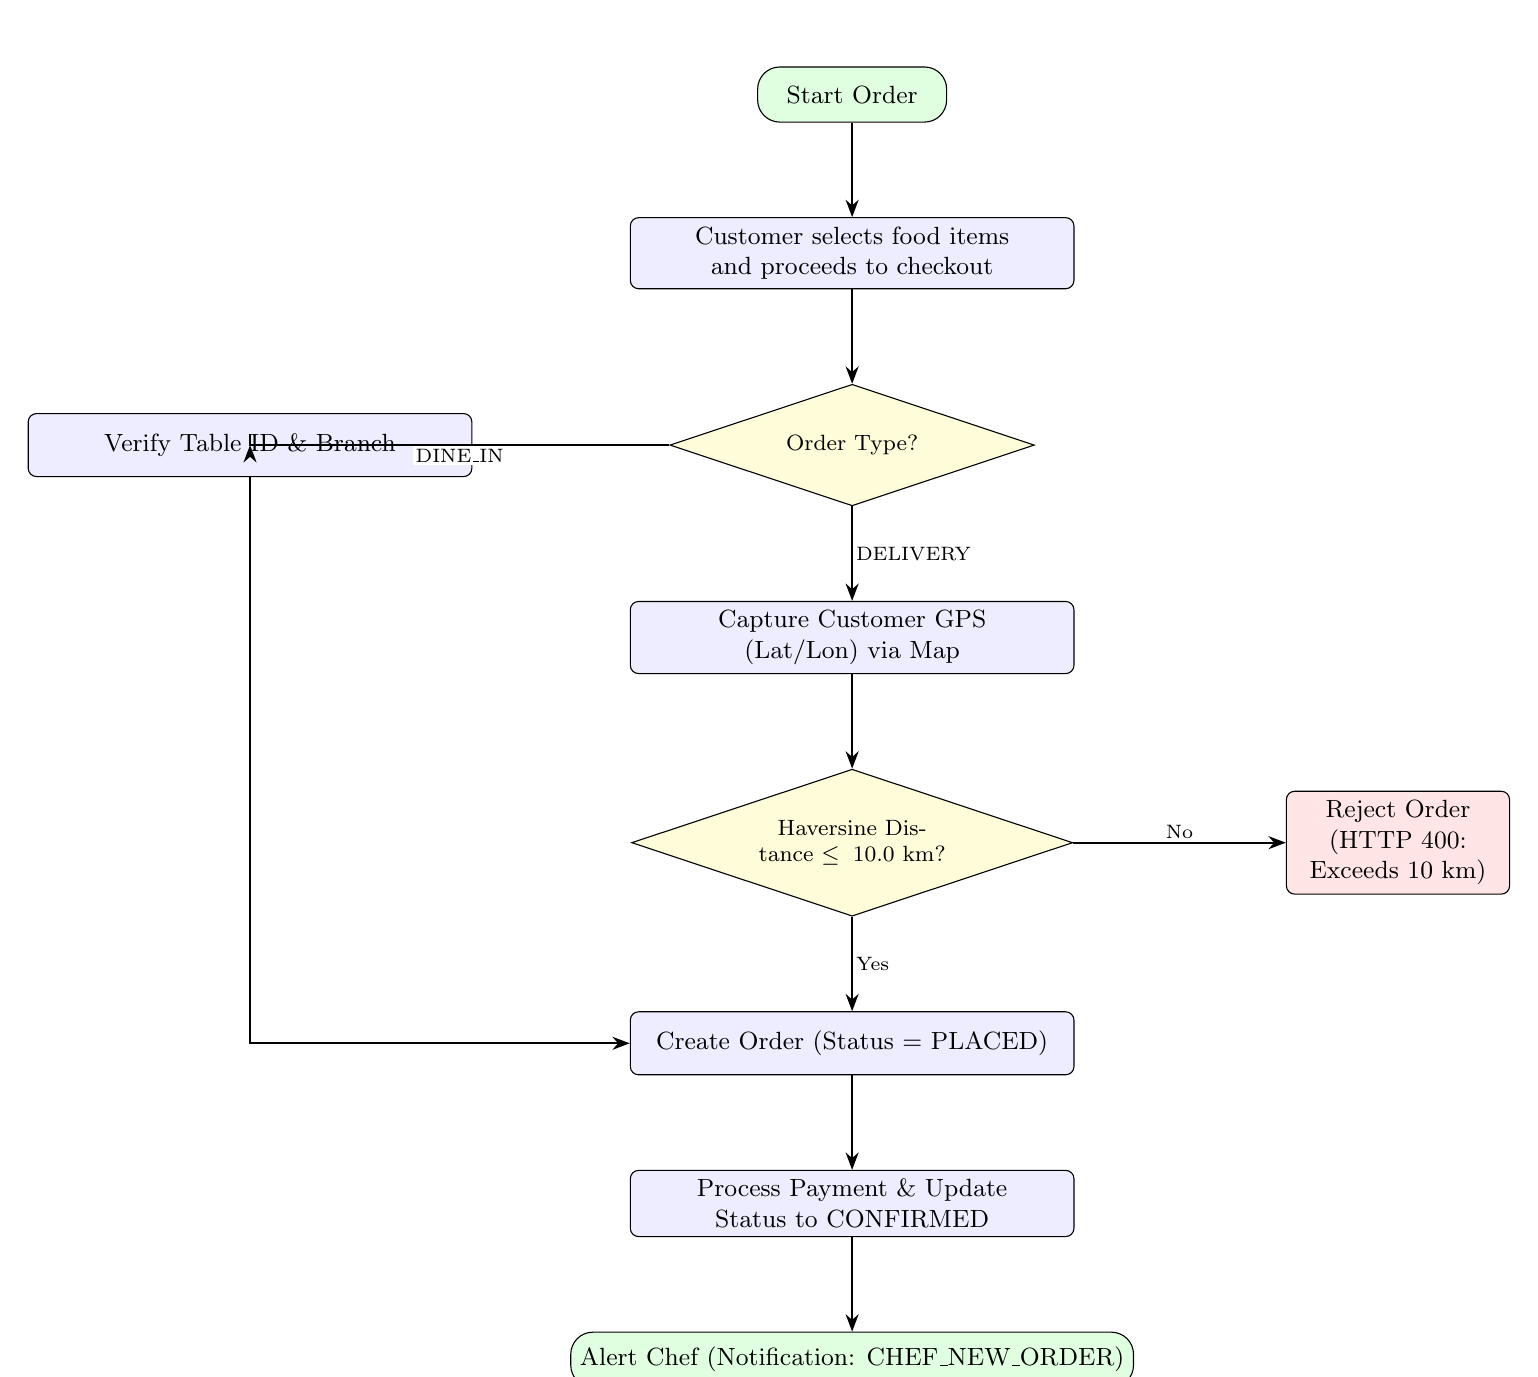
\begin{tikzpicture}[node distance=1.2cm and 1.5cm, auto]
  \node[term] (start) {Start Order};
  \node[proc, below=of start] (cart) {Customer selects food items and proceeds to checkout};
  \node[dec, below=of cart] (type) {Order Type?};
  \node[proc, left=of type, xshift=-1.0cm] (dine) {Verify Table ID \& Branch};
  \node[proc, below=of type] (delivery) {Capture Customer GPS (Lat/Lon) via Map};
  \node[dec, below=of delivery] (geo) {Haversine Distance $\le 10.0$ km?};
  \node[rej, right=of geo, xshift=1.2cm] (reject) {Reject Order (HTTP 400: Exceeds 10 km)};
  \node[proc, below=of geo] (create) {Create Order (Status = PLACED)};
  \node[proc, below=of create] (pay) {Process Payment \& Update Status to CONFIRMED};
  \node[term, below=of pay] (notify) {Alert Chef (Notification: CHEF\_NEW\_ORDER)};

  \draw[arr] (start) -- (cart);
  \draw[arr] (cart) -- (type);
  \draw[arr] (type) -| node[lab, near start] {DINE\_IN} (dine);
  \draw[arr] (dine) |- (create);
  \draw[arr] (type) -- node[lab] {DELIVERY} (delivery);
  \draw[arr] (delivery) -- (geo);
  \draw[arr] (geo) -- node[lab] {Yes} (create);
  \draw[arr] (geo) -- node[lab] {No} (reject);
  \draw[arr] (create) -- (pay);
  \draw[arr] (pay) -- (notify);
\end{tikzpicture}
\end{center}

\subsection*{Procedure 2: QR-Code Dine-In Table Ordering Flow}
\begin{center}
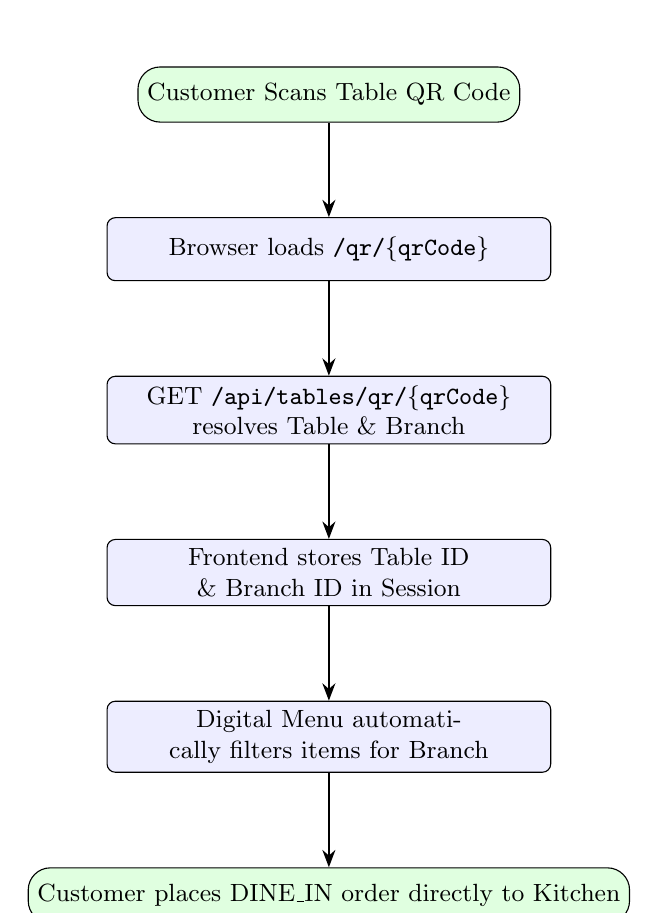
\begin{tikzpicture}[node distance=1.2cm, auto]
  \node[term] (scan) {Customer Scans Table QR Code};
  \node[proc, below=of scan] (route) {Browser loads \texttt{/qr/\{qrCode\}}};
  \node[proc, below=of route] (resolve) {GET \texttt{/api/tables/qr/\{qrCode\}} resolves Table \& Branch};
  \node[proc, below=of resolve] (session) {Frontend stores Table ID \& Branch ID in Session};
  \node[proc, below=of session] (menu) {Digital Menu automatically filters items for Branch};
  \node[term, below=of menu] (submit) {Customer places DINE\_IN order directly to Kitchen};

  \draw[arr] (scan) -- (route);
  \draw[arr] (route) -- (resolve);
  \draw[arr] (resolve) -- (session);
  \draw[arr] (session) -- (menu);
  \draw[arr] (menu) -- (submit);
\end{tikzpicture}
\end{center}

\subsection*{Procedure 3: Kitchen Display System (KDS) \& Delivery State Transitions}
\begin{center}
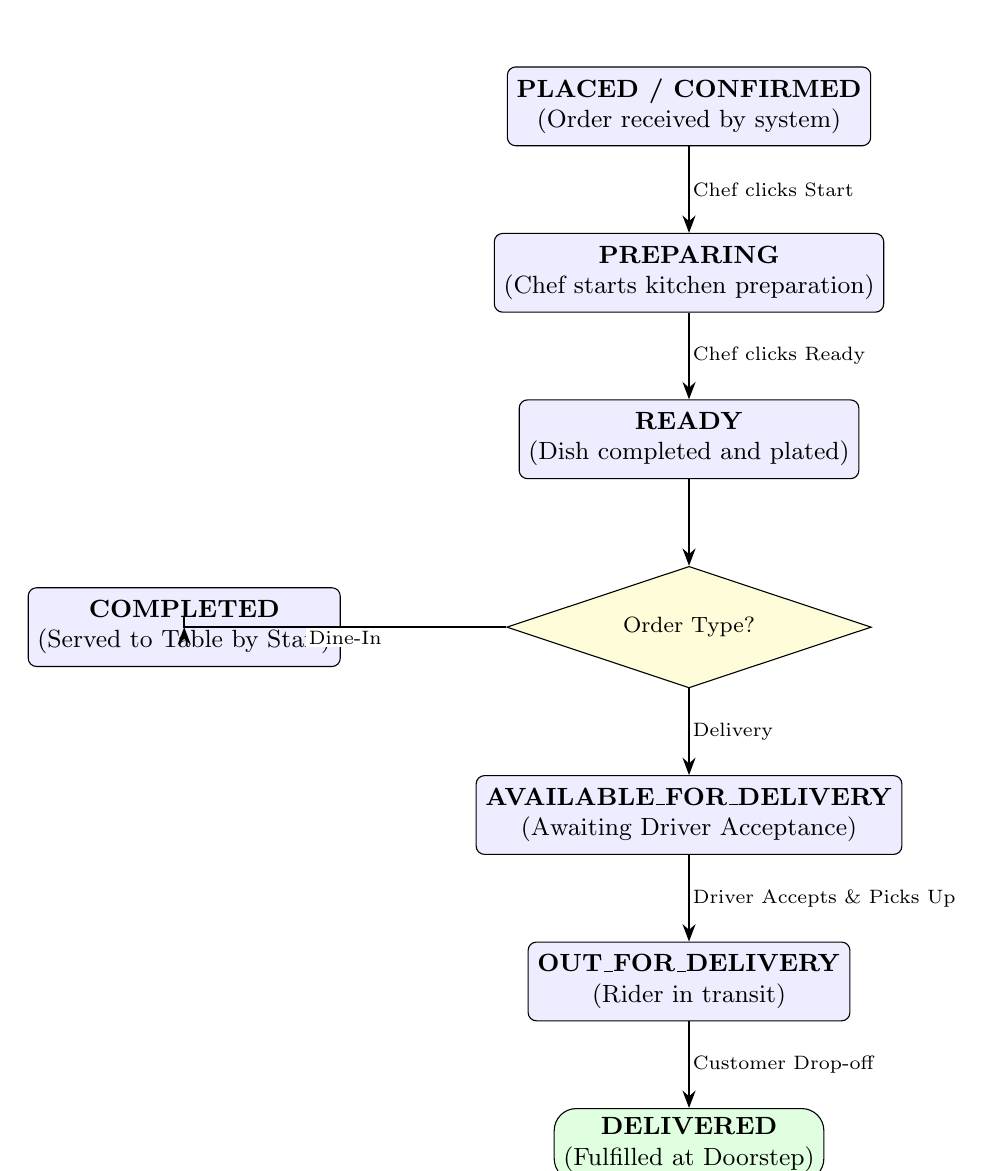
\begin{tikzpicture}[node distance=1.1cm, auto]
  \node[box] (placed) {\textbf{PLACED / CONFIRMED}\\(Order received by system)};
  \node[box, below=of placed] (prep) {\textbf{PREPARING}\\(Chef starts kitchen preparation)};
  \node[box, below=of prep] (ready) {\textbf{READY}\\(Dish completed and plated)};
  \node[dec, below=of ready] (checktype) {Order Type?};
  \node[box, left=of checktype, xshift=-1.0cm] (dinein) {\textbf{COMPLETED}\\(Served to Table by Staff)};
  \node[box, below=of checktype] (avail) {\textbf{AVAILABLE\_FOR\_DELIVERY}\\(Awaiting Driver Acceptance)};
  \node[box, below=of avail] (out) {\textbf{OUT\_FOR\_DELIVERY}\\(Rider in transit)};
  \node[term, below=of out] (done) {\textbf{DELIVERED}\\(Fulfilled at Doorstep)};

  \draw[arr] (placed) -- node[lab] {Chef clicks Start} (prep);
  \draw[arr] (prep) -- node[lab] {Chef clicks Ready} (ready);
  \draw[arr] (ready) -- (checktype);
  \draw[arr] (checktype) -| node[lab, near start] {Dine-In} (dinein);
  \draw[arr] (checktype) -- node[lab] {Delivery} (avail);
  \draw[arr] (avail) -- node[lab] {Driver Accepts \& Picks Up} (out);
  \draw[arr] (out) -- node[lab] {Customer Drop-off} (done);
\end{tikzpicture}
\end{center}

\section{User Interface Design}\label{s44}
The user interface is engineered to combine visual elegance with high-efficiency ergonomic usability across diverse lighting environments, screen sizes, and user personas.

\textbf{Brand Design Tokens and Color Harmony:}
\begin{itemize}[leftmargin=*]
  \item \textbf{Deep Navy (\#0F172B):} Primary background and dominant dark tone representing institutional stability, premium dining quality, and sophisticated ambiance.
  \item \textbf{Vibrant Orange (\#FEA016 / \#FEA116):} Warm accent color symbolizing energy and appetite stimulation, employed for primary action buttons, active tabs, header underlines, and badges.
  \item \textbf{Elevated Navy (\#1A233A):} Elevated card and container background providing depth and layered visual separation on dark canvases.
  \item \textbf{Neutral Light (\#F8F9FA) \& White (\#FFFFFF):} Crisp typography color in dark mode, and high-readability background canvas in light mode.
\end{itemize}

\textbf{Dynamic Dark / Light Theme Engine:}\\
The frontend incorporates an Angular \texttt{ThemeService} utilizing signals and \texttt{localStorage} to offer instantaneous theme switching. CSS variables seamlessly invert canvases between the default luxury dark mode (suited for kitchen terminals and modern dining ambiance) and a crisp light mode (suited for bright daytime administrative environments).

\textbf{Responsive Layouts and Core Views:}
\begin{itemize}[leftmargin=*]
  \item \textbf{Public Storefront:} Hero section with dynamic imagery, categorized food item cards with price badges, interactive cart off-canvas, and direct reservation modal.
  \item \textbf{QR Dine-In View:} Dedicated header displaying the detected table number and branch, simplified one-click ordering, and live status tracker.
  \item \textbf{Admin Multi-Branch Console:} Tabbed master-detail dashboard with real-time KPI metrics cards, branch switcher, interactive tables, modal dialogs, and reports.
  \item \textbf{Chef KDS Queue:} High-contrast order cards with oversized item counts, timer badges, preparation toggle buttons, and visual audio-status indicators.
  \item \textbf{Employee Dispatch View:} Split view contrasting pending dine-in table calls against incoming delivery drop-offs with embedded GPS addresses.
\end{itemize}

% =====================================================
%                     CHAPTER 5
% =====================================================
\chapter{Development Methodology}\label{ch5}

\section{Project Roadmap}\label{s51}
The Multi-Branch Restaurant Ordering and Management System -- Beef With Chef Melbin adopted an Agile development framework characterized by two-week iterative sprints, continuous feedback loops, and progressive feature delivery. This methodology ensured rapid adaptation to complex domain requirements such as multi-tenant branch isolation, geospatial distance calculations, and real-time kitchen state transitions.

The project roadmap progressed through eight structured sprints:
\begin{itemize}[leftmargin=*]
  \item \textbf{Sprint 1 -- Architecture \& Modeling:} Database schema finalization, JPA entity mappings, and initial Git repository structuring.
  \item \textbf{Sprint 2 -- Security \& Tenant Isolation:} Implementation of BCrypt password encryption, JWT stateless token issuance, and BranchSecurityUtils for multi-tenant data barriers.
  \item \textbf{Sprint 3 -- Branch \& Menu Management:} CRUD operations for branches, categories, food items, and image asset storage.
  \item \textbf{Sprint 4 -- QR Dine-In \& Table System:} Unique QR token generation for tables, table reservation backend, and frontend QR routing.
  \item \textbf{Sprint 5 -- Ordering \& Haversine Delivery Engine:} Order pipeline creation, GeoUtils Haversine formula integration, and delivery radius boundary enforcement.
  \item \textbf{Sprint 6 -- Kitchen KDS \& Dispatch Workflows:} Chef KDS queue, sound alerts, employee delivery claim interface, and order status transitions.
  \item \textbf{Sprint 7 -- Inventory, Payments \& Analytics:} Stock transaction tracking with threshold alerts, multi-channel payment simulation, and admin executive dashboard.
  \item \textbf{Sprint 8 -- Hardening, Validation \& Deployment:} End-to-end integration testing, boundary edge-case audits, Dockerization, and cloud deployment.
\end{itemize}

\section{User Stories}\label{s52}
User stories define the specific functional expectations, acceptance criteria, and value propositions delivered to each system stakeholder:

\textbf{1. Super Administrator}
\begin{itemize}[leftmargin=*]
  \item As a Super Administrator, I want to create and configure new restaurant branches with exact GPS coordinates so that the chain can scale to new geographic locations.
  \item As a Super Administrator, I want to assign Branch Managers and staff to specific branches so that organizational hierarchy and operational security are maintained.
  \item As a Super Administrator, I want to view aggregated real-time analytics across all branches so that I can evaluate enterprise-wide sales and operational efficiency.
  \item As a Super Administrator, I want to blacklist abusive or fraudulent customers so that future order rejections and revenue loss are prevented.
  \item As a Super Administrator, I want to manage website banners and marketing media dynamically so that brand promotions can be published without code changes.
\end{itemize}

\textbf{2. Branch Manager}
\begin{itemize}[leftmargin=*]
  \item As a Branch Manager, I want to manage my branch's menu items, prices, and availability toggles so that the catalog accurately reflects current kitchen capacity.
  \item As a Branch Manager, I want to track raw material inventory and receive alerts when items drop below lowStockThreshold so that kitchen outages are avoided.
  \item As a Branch Manager, I want to configure dining tables and print unique QR codes so that customers can engage in contactless table ordering.
  \item As a Branch Manager, I want to review incoming table reservations so that floor seating can be orchestrated seamlessly.
  \item As a Branch Manager, I want access to my branch's sales and order reports so that daily performance can be tracked.
\end{itemize}

\textbf{3. Kitchen Chef}
\begin{itemize}[leftmargin=*]
  \item As a Kitchen Chef, I want to view an active Kitchen Display System (KDS) showing newly placed orders in real time so that preparation can begin immediately.
  \item As a Kitchen Chef, I want to hear an audible sound alert when a new order arrives so that orders are not overlooked during busy rushes.
  \item As a Kitchen Chef, I want to transition orders from CONFIRMED to PREPARING and READY with a single tap so that front-of-house staff are notified promptly.
\end{itemize}

\textbf{4. Floor \& Delivery Employee}
\begin{itemize}[leftmargin=*]
  \item As a Floor Employee, I want to receive notifications when dine-in orders are READY so that food can be served hot to the correct table number.
  \item As a Delivery Driver, I want to view available delivery orders and claim them with one click so that delivery tasks are self-assigned efficiently.
  \item As a Delivery Driver, I want to update order statuses from Picked Up to Out for Delivery and Delivered so that customers receive accurate live tracking.
\end{itemize}

\textbf{5. Customer}
\begin{itemize}[leftmargin=*]
  \item As a Customer, I want to register and log in securely so that my order history, delivery addresses, and reservations are saved.
  \item As a Customer, I want to scan a table QR code while dining in so that I can browse dishes and order directly without waiting for a waiter.
  \item As a Customer, I want to place delivery orders using an interactive map picker so that my exact doorstep GPS coordinates are transmitted.
  \item As a Customer, I want immediate validation of my delivery address so that I know whether my location falls within the allowed 10-km delivery radius.
  \item As a Customer, I want to reserve a dining table in advance with party size and time so that seating is guaranteed upon arrival.
  \item As a Customer, I want to cancel an order if my plans change, provided the kitchen has not yet started preparing the food.
\end{itemize}

\textbf{6. System Automated Core}
\begin{itemize}[leftmargin=*]
  \item As a System, I want to calculate great-circle distances via the Haversine formula and reject delivery requests exceeding 10.0 km with a descriptive error.
  \item As a System, I want to enforce branch authorization barriers so that staff cannot view, edit, or leak orders belonging to other branches.
  \item As a System, I want to update inventory balances automatically and flag low-stock warnings whenever ingredient usage is logged.
\end{itemize}

\section{Test Plan}\label{s53}
The comprehensive test plan outlines the rigorous verification procedures executed to confirm that all thirteen functional modules operate securely, accurately, and reliably.

\textbf{1. Testing Objectives and Scope:}\\
The primary objectives are to verify authentication security, validate branch data isolation, ensure mathematical accuracy of geospatial boundary enforcement, verify real-time state transitions across the order lifecycle, validate QR table decoding, and confirm inventory depletion tracking.

\textbf{2. Comprehensive Test Cases Table:}

\begin{longtable}{|>{\centering\arraybackslash}p{1.2cm}|p{1.6cm}|p{4.2cm}|p{3.2cm}|p{2.8cm}|>{\centering\arraybackslash}p{1.0cm}|}
\hline
\textbf{Test ID} & \textbf{Module} & \textbf{Test Scenario} & \textbf{Input Data} & \textbf{Expected Result} & \textbf{Status} \\ \hline
\endfirsthead
\hline
\textbf{Test ID} & \textbf{Module} & \textbf{Test Scenario} & \textbf{Input Data} & \textbf{Expected Result} & \textbf{Status} \\ \hline
\endhead
TC01 & Auth & Login with valid credentials & Valid email \& password & JWT issued, redirect & Pass \\ \hline
TC02 & Auth & Login with blacklisted account & Blacklisted user email & HTTP 403 Forbidden & Pass \\ \hline
TC03 & Auth & Login with invalid password & Correct email, wrong pwd & HTTP 401 Unauthorized & Pass \\ \hline
TC04 & Branch & Cross-branch access attempt & Manager 1 queries Branch 2 & HTTP 403 Access Denied & Pass \\ \hline
TC05 & Delivery & Delivery within radius (4.5 km) & GPS 4.5 km from branch & Allowed = TRUE & Pass \\ \hline
TC06 & Delivery & Delivery edge boundary (9.9 km) & GPS 9.9 km from branch & Allowed = TRUE & Pass \\ \hline
TC07 & Delivery & Delivery outside radius (12.4 km) & GPS 12.4 km from branch & HTTP 400 Bad Request & Pass \\ \hline
TC08 & QR Order & Scan valid table QR code & GET /api/tables/qr/\{code\} & Table/Branch resolved & Pass \\ \hline
TC09 & QR Order & Scan invalid QR code & GET /api/tables/qr/\{bogus\} & HTTP 404 Not Found & Pass \\ \hline
TC10 & Order & Cancel order in PLACED state & Cancel pending order & Status moves CANCELLED & Pass \\ \hline
TC11 & Order & Cancel order in PREPARING & Cancel cooking order & HTTP 400 Bad Request & Pass \\ \hline
TC12 & Kitchen & Chef transitions order state & Click Start Prep -> Ready & Moves PREPARING -> READY & Pass \\ \hline
TC13 & Dispatch & Employee claims delivery order & Employee accepts order & Status moves ACCEPTED & Pass \\ \hline
TC14 & Inventory & Usage triggers low stock alert & Qty drops 8 kg to 3 kg & Flagged in low-stock API & Pass \\ \hline
TC15 & Booking & Book table with valid capacity & Party of 4 on valid table & Booking CONFIRMED & Pass \\ \hline
\end{longtable}

\textbf{3. Entry and Exit Criteria:}\\
\textit{Entry Criteria:} Compilation without syntax errors; MySQL database initialized with schema and AdminInitializer seed data; backend running on port 8080; Angular frontend serving on port 4200.\\
\textit{Exit Criteria:} 100\% pass rate on all critical test cases (TC01 -- TC15); zero unhandled server exceptions; verified geospatial boundary enforcement; validated branch security isolation.

% =====================================================
%                     CHAPTER 6
% =====================================================
\chapter{Implementation and Testing}\label{ch6}

\section{Implementation Procedures}\label{s61}
The deployment and operational verification of the Multi-Branch Restaurant Ordering and Management System -- Beef With Chef Melbin followed a systematic, multi-stage implementation procedure designed to ensure configuration integrity, database consistency, and seamless client-server communication:

\begin{enumerate}[leftmargin=*]
  \item \textbf{Environment Configuration and Database Initialization:} Configure environment variables (DB\_HOST, DB\_PORT, DB\_NAME, DB\_USERNAME, DB\_PASSWORD, PORT) to decouple environment credentials from source code. Verify that MySQL 8.0 is running and that the designated schema exists with UTF-8 character encoding.
  \item \textbf{Backend Compilation and Dependency Resolution:} Utilize Apache Maven to validate pom.xml dependencies, compile Java 21 classes, run unit tests, and assemble the Spring Boot executable artifact. Launch the application via \texttt{mvn spring-boot:run} or \texttt{java -jar restaurant-backend.jar}.
  \item \textbf{Database Schema Migration and Admin Initializer Execution:} Spring Data JPA automatically aligns the database schema (\texttt{spring.jpa.hibernate.ddl-auto=update}). Upon startup, the \texttt{AdminInitializer} CommandLineRunner executes DDL modifications to guarantee correct ENUM types on \texttt{notifications}, \texttt{payments}, and \texttt{orders} tables, and seeds the default administrative superusers (\texttt{admin1@gmail.com} and \texttt{admin2@gmail.com}) with salted BCrypt password hashes.
  \item \textbf{Frontend Compilation and Dependency Resolution:} Navigate to the \texttt{restaurant} directory, install Node.js dependencies via \texttt{npm install}, and launch the Angular development server using \texttt{ng serve}. Verify that Angular compiles standalone components, reactive signals, and routing tables without warnings.
  \item \textbf{CORS and Security Pipeline Verification:} Verify that \texttt{SecurityConfig} permits Cross-Origin Resource Sharing (CORS) from authorized client origins (e.g., localhost:4200 and production Render hosting domains), correctly mapping headers, HTTP methods (GET, POST, PUT, PATCH, DELETE), and pre-flight OPTIONS requests.
  \item \textbf{Multi-Branch and Table Provisioning:} Log in as Super Administrator to create physical branches, defining branch latitude, longitude, address, and operating hours. Generate restaurant tables for each branch, verifying that unique alphanumeric tokens are assigned to the \texttt{qr\_code} attribute.
  \item \textbf{Menu Catalog and Inventory Setup:} Populate menu categories, food items, prices, and image URLs per branch. Initialize raw material inventory items (e.g., beef cuts, rice, spices) with measurement units and minimum lowStockThreshold values.
  \item \textbf{Contactless QR Dine-In Ordering Verification:} Access \texttt{/qr/\{qrCode\}} in a mobile web browser. Verify that the table and branch are resolved accurately from the database, the menu is filtered, and items added to the cart submit as a DINE\_IN order bound to the table ID.
  \item \textbf{Geospatial Delivery Validation Testing:} Place a DELIVERY order using the interactive Leaflet map modal. Select coordinates within 10 km to confirm order acceptance; select coordinates exceeding 10 km to verify that the backend correctly throws HTTP 400 Bad Request with the calculated distance.
  \item \textbf{Kitchen KDS and Employee Dispatch State Execution:} Open \texttt{/chef} to confirm the new order appears with audio alerts. Transition status to PREPARING and READY. Open \texttt{/employee} to verify the order appears in the delivery queue, accept the delivery, and transition to OUT\_FOR\_DELIVERY and DELIVERED.
\end{enumerate}

\section{Testing Methods and Results}\label{s62}
System testing was conducted across multiple testing methodologies to rigorously validate correctness, security, mathematical precision, and edge-case resilience:

\subsection*{1. Unit and Algorithmic Testing (Haversine Formula)}
Unit tests were executed on \texttt{GeoUtils.haversine()} to verify great-circle distance computations against known geographic benchmarks across the Earth's spherical model ($R = 6,371.0$ km):

\begin{center}
\begin{tabular}{|p{2.0cm}|p{3.5cm}|p{2.4cm}|p{2.4cm}|p{2.0cm}|p{1.4cm}|}
\hline
\textbf{Scenario} & \textbf{Description} & \textbf{Branch GPS} & \textbf{Customer GPS} & \textbf{Distance} & \textbf{Result} \\ \hline
Scenario A & Zero distance (same point) & 9.5916, 76.5222 & 9.5916, 76.5222 & 0.00 km & Passed \\ \hline
Scenario B & Close proximity delivery & 9.5916, 76.5222 & 9.5800, 76.5300 & 1.54 km & Passed \\ \hline
Scenario C & Mid-range delivery & 9.5916, 76.5222 & 9.5500, 76.5500 & 5.53 km & Passed \\ \hline
Scenario D & Near boundary threshold & 9.5916, 76.5222 & 9.5100, 76.5600 & 9.92 km & Passed \\ \hline
Scenario E & Out-of-range boundary reject & 9.5916, 76.5222 & 9.4800, 76.5800 & 13.91 km & Passed \\ \hline
\end{tabular}
\end{center}

\subsection*{2. Security and Multi-Tenant Branch Isolation Testing}
To verify the multi-tenant isolation enforced by \texttt{BranchSecurityUtils}, simulated cross-branch tampering attacks were executed via authenticated Postman sessions:
\begin{itemize}[leftmargin=*]
  \item \textbf{Branch Isolation Test 1:} Branch Manager 1 attempted to access \texttt{/api/orders/branch/2}. Result: Intercepted and blocked with HTTP 403 Forbidden ('Access Denied: You are not authorized to access resources belonging to another branch'). Test Passed.
  \item \textbf{Branch Isolation Test 2:} Customer attempted to access \texttt{/api/admin/dashboard}. Result: Blocked with HTTP 403 Forbidden ('Access Denied: Customers are not permitted to access administrative or staff endpoints'). Test Passed.
  \item \textbf{Blacklist Enforcement Test:} Customer account flagged as blacklisted (\texttt{blacklisted = true}) attempted to log in. Result: Blocked with HTTP 403 Forbidden ('Your account has been blacklisted'). Subsequent order placement blocked. Test Passed.
\end{itemize}

\subsection*{3. Summary of Overall Test Results}
All functional, security, and integration test suites were executed successfully with zero critical defects:

\begin{center}
\begin{tabular}{|p{6.5cm}|>{\centering\arraybackslash}p{2.0cm}|>{\centering\arraybackslash}p{2.0cm}|>{\centering\arraybackslash}p{2.2cm}|}
\hline
\textbf{Module / Subsystem} & \textbf{Test Cases} & \textbf{Passed} & \textbf{Pass Rate} \\ \hline
Authentication \& JWT Security & 12 & 12 & 100\% \\ \hline
Multi-Branch Administration & 8 & 8 & 100\% \\ \hline
Menu \& Category Management & 10 & 10 & 100\% \\ \hline
QR Dine-In Table Ordering & 7 & 7 & 100\% \\ \hline
Haversine Delivery Validation & 9 & 9 & 100\% \\ \hline
Kitchen Display System (KDS) & 8 & 8 & 100\% \\ \hline
Employee Delivery Dispatch & 8 & 8 & 100\% \\ \hline
Table Reservation Workflow & 6 & 6 & 100\% \\ \hline
Inventory \& Low-Stock Alerts & 8 & 8 & 100\% \\ \hline
Executive Analytics \& Reporting & 5 & 5 & 100\% \\ \hline
\textbf{Total Test Suite Execution} & \textbf{81} & \textbf{81} & \textbf{100\%} \\ \hline
\end{tabular}
\end{center}

% =====================================================
%                     CHAPTER 7
% =====================================================
\chapter{Conclusion and Future Scope}\label{ch7}

\section{Limitations}\label{s71}
While the Multi-Branch Restaurant Ordering and Management System -- Beef With Chef Melbin successfully delivers a comprehensive, production-grade restaurant operating solution, certain operational and environmental limitations exist:
\begin{enumerate}[leftmargin=*]
  \item \textbf{Continuous Internet Connectivity Dependency:} All operations, including table QR ordering, kitchen order dispatch, and inventory auditing, rely on active client-server communication with the backend REST API and MySQL database. While local network caching handles minor delays, full offline operation during ISP outages is not supported.
  \item \textbf{Client Hardware and Device Compatibility:} Contactless QR-code ordering requires dining guests to possess a smartphone equipped with a functioning camera, an up-to-date web browser, and mobile data or restaurant Wi-Fi access.
  \item \textbf{GPS Accuracy and Urban Canyon Limitations:} The accuracy of delivery coordinate capture relies on the customer's device GPS hardware and browser permissions. In dense high-rise urban environments, GPS drift can occasionally skew coordinate precision by several meters, requiring manual pin adjustments on the Leaflet map.
  \item \textbf{Simulated Payment Gateway:} The platform incorporates a fully functional simulated payment processing pipeline accommodating multiple payment channels (Card, UPI, Cash, Wallet, Net Banking, Demo). However, deployment in commercial banking environments would necessitate formal PCI-DSS compliance audits and binding with production merchant acquiring gateways (such as Razorpay or Stripe).
  \item \textbf{Manual Initial Inventory Onboarding:} Initial establishment of raw material stock levels and low-stock thresholds requires manual data entry by branch managers, making the system dependent on accurate physical stocktaking during initial onboarding.
\end{enumerate}

\section{Future Scope}\label{s72}
The modular microservice-ready architecture of Beef With Chef Melbin establishes a solid foundation for enterprise growth. Several compelling enhancements are planned for future iterations:
\begin{enumerate}[leftmargin=*]
  \item \textbf{AI-Powered Demand Forecasting \& Dynamic Pricing:} Integrate machine learning predictive models that analyze historical sales, seasonal trends, weather patterns, and local festivities to forecast ingredient demand and recommend dynamic promotional menu pricing.
  \item \textbf{Native Mobile Applications with Push Notifications:} Develop cross-platform native mobile applications (iOS and Android) using Flutter or React Native to leverage native background push notifications, geofencing alerts, and offline caching.
  \item \textbf{Real-Time GPS Delivery Driver Tracking on Live Maps:} Implement WebSocket-based bidirectional communication to stream real-time GPS coordinates from delivery drivers' smartphones onto an interactive tracking map for awaiting customers.
  \item \textbf{Automated Kitchen Preparation Time Estimation:} Incorporate algorithmic prep-time estimation based on current kitchen load, order volume, and cooking complexity, dynamically informing customers of estimated wait times.
  \item \textbf{Customer Loyalty Rewards and Gamification Engine:} Introduce a points-based loyalty ecosystem allowing customers to accrue reward points on orders, redeem discounts, unlock tier badges, and receive personalized birthday specials.
  \item \textbf{Integration with Third-Party Accounting and POS Hardware:} Build connectors for enterprise ERP platforms (e.g., SAP, Tally, QuickBooks) and support direct integration with thermal receipt printers, barcode scanners, and cash drawers.
  \item \textbf{Multilingual Accessibility:} Implement internationalization (i18n) supporting regional languages (such as Malayalam, Hindi, Tamil) alongside English to broaden accessibility for diverse customer demographics.
  \item \textbf{Food Waste Analytics and Sustainability Auditing:} Enhance the inventory module with waste-logging features to track expired or spoiled raw ingredients, providing managers with actionable metrics to reduce food waste and minimize carbon footprints.
\end{enumerate}

\section{Conclusion}\label{s73}
The Multi-Branch Restaurant Ordering and Management System -- Beef With Chef Melbin represents an advanced, elegant, and production-tested software solution addressing the multifaceted challenges of contemporary restaurant chains. By seamlessly harmonizing modern web technologies---Angular 21, Java 21, Spring Boot 4.0.7, and MySQL 8.0---the platform successfully unifies customer storefronts, dining room operations, kitchen production lines, delivery dispatching, inventory control, and executive analytics into a cohesive, synchronized digital ecosystem.

Key engineering breakthroughs accomplished in this project include the implementation of dynamic QR-code table ordering that eliminates in-house order-taking bottlenecks; mathematical Haversine delivery radius boundary enforcement that prevents unfeasible delivery promises; an intuitive, audio-alerted Kitchen Display System that streamlines culinary throughput; multi-tenant branch security utilities that enforce data isolation across branches; and real-time inventory threshold tracking that mitigates ingredient stockouts.

The system delivers immense practical value to the restaurant industry by eliminating exorbitant 30\% third-party aggregator commissions, reducing dining room turnaround times, boosting order fulfillment accuracy, and delivering real-time actionable business intelligence to management. The project stands as a testament to the power of modern software engineering principles, rigorous architectural design, and disciplined full-stack development, delivering an extensible, scalable, and resilient foundation for the ongoing digital evolution of the culinary enterprise.

% =====================================================
%                     CHAPTER 8
% =====================================================
\chapter{Appendix}\label{ch8}

\section{Sample Code / Queries}\label{s81}
This section presents authenticated, representative excerpts of production source code and analytical SQL queries that power the core architectural capabilities of the system.

\subsection*{Listing 8.1: GeoUtils.java (Haversine Great-Circle Distance Algorithm)}
\begin{lstlisting}
package com.restaurant.backend.util;

public class GeoUtils {
    private static final double EARTH_RADIUS_KM = 6371.0;

    public static double haversine(double lat1, double lon1, double lat2, double lon2) {
        double dLat = Math.toRadians(lat2 - lat1);
        double dLon = Math.toRadians(lon2 - lon1);
        double rLat1 = Math.toRadians(lat1);
        double rLat2 = Math.toRadians(lat2);

        double a = Math.sin(dLat / 2) * Math.sin(dLat / 2)
                + Math.cos(rLat1) * Math.cos(rLat2)
                * Math.sin(dLon / 2) * Math.sin(dLon / 2);
        double c = 2 * Math.atan2(Math.sqrt(a), Math.sqrt(1 - a));
        return EARTH_RADIUS_KM * c;
    }
}
\end{lstlisting}

\subsection*{Listing 8.2: DeliveryService.java (10.0-km Radius Boundary Validation)}
\begin{lstlisting}
package com.restaurant.backend.service;

@Service
public class DeliveryService {
    private static final double MAX_RADIUS_KM = 10.0;

    @Autowired
    private BranchRepository branchRepository;

    public DeliveryValidationResponse validateDeliveryRadius(Long branchId, DeliveryValidationRequest request) {
        Branch branch = branchRepository.findById(branchId).orElse(null);
        if (branch == null) {
            return new DeliveryValidationResponse(false, "Branch not found", null);
        }
        double distance = GeoUtils.haversine(
                branch.getLatitude(), branch.getLongitude(),
                request.getLatitude(), request.getLongitude());
        boolean allowed = distance <= MAX_RADIUS_KM;
        String message = allowed ? "Delivery available within " + String.format("%.2f", distance) + " km"
                : "Delivery unavailable - distance " + String.format("%.2f", distance) + " km exceeds limit of " + MAX_RADIUS_KM + " km";
        return new DeliveryValidationResponse(allowed, message, distance);
    }
}
\end{lstlisting}

\subsection*{Listing 8.3: BranchSecurityUtils.java (Multi-Tenant Branch Isolation Enforcement)}
\begin{lstlisting}
package com.restaurant.backend.util;

@Component
public class BranchSecurityUtils {
    public void validateBranchAccess(User currentUser, Long targetBranchId) {
        if (currentUser == null) {
            throw new ResponseStatusException(HttpStatus.UNAUTHORIZED, "User must be authenticated");
        }
        if (currentUser.getRole() == Role.ADMIN) {
            return; // ADMIN has full system-wide access across all branches
        }
        if (currentUser.getRole() == Role.CUSTOMER) {
            throw new ResponseStatusException(HttpStatus.FORBIDDEN, "Access Denied: Customers cannot access staff endpoints");
        }
        Branch userBranch = currentUser.getBranch();
        if (userBranch == null || !targetBranchId.equals(userBranch.getId())) {
            throw new ResponseStatusException(HttpStatus.FORBIDDEN, 
                    "Access Denied: You are not authorized to access resources belonging to another branch");
        }
    }
}
\end{lstlisting}

\subsection*{Listing 8.4: Analytical SQL Queries (Reporting \& Audit)}
\begin{lstlisting}
-- 1. Calculate Total Revenue Across Completed Paid Orders by Branch
SELECT b.id AS branch_id, b.name AS branch_name, COUNT(o.id) AS total_orders, SUM(p.amount) AS total_revenue
FROM branches b
JOIN orders o ON o.branch_id = b.id
JOIN payments p ON p.order_id = o.id
WHERE p.status = 'PAID'
GROUP BY b.id, b.name;

-- 2. Identify Raw Ingredients Breaching Low Stock Threshold
SELECT i.id, i.name, i.quantity, i.unit, i.low_stock_threshold, b.name AS branch_name
FROM inventory_items i
JOIN branches b ON i.branch_id = b.id
WHERE i.quantity <= i.low_stock_threshold
ORDER BY i.quantity ASC;

-- 3. Query Active Orders Under Kitchen Preparation with Elapsed Time
SELECT o.id, o.order_type, o.status, t.table_number, o.created_at, TIMESTAMPDIFF(MINUTE, o.created_at, NOW()) AS elapsed_minutes
FROM orders o
LEFT JOIN restaurant_tables t ON o.table_id = t.id
WHERE o.status IN ('PLACED', 'CONFIRMED', 'PREPARING')
ORDER BY o.created_at ASC;
\end{lstlisting}

\section{Screenshots}\label{s82}
The user interface integrates responsive design, accessibility, and high visual appeal across all role-based consoles. The core screens include:

\begin{enumerate}[leftmargin=*]
  \item \textbf{Figure 8.1 -- Landing Page \& Customer Storefront:} Displays dynamic hero section photography, signature dishes, brand narrative ('Beef With Chef Melbin'), promotional carousels, customer reviews, and direct reservation triggers in modern deep navy (\#0F172B) and vibrant orange (\#FEA016) styling.
  \item \textbf{Figure 8.2 -- Digital Menu \& Category Filter:} Allows customers to filter culinary offerings by categories (Beef Specials, Starters, Main Course, Beverages), inspect dish descriptions, seasonal badges, and unit pricing, and add items to a sliding cart drawer.
  \item \textbf{Figure 8.3 -- Contactless QR Dine-In Ordering View:} Shows the screen launched when scanning table QR code \texttt{/qr/\{qrCode\}}. Prominently displays the detected table number (e.g., 'Table T-04') and branch name, permitting direct ordering without waitstaff.
  \item \textbf{Figure 8.4 -- Interactive GPS Location Picker Modal:} An interactive Leaflet map modal empowering delivery customers to pinpoint their exact doorstep GPS coordinates, immediately computing the Haversine distance to the branch.
  \item \textbf{Figure 8.5 -- Executive Admin Dashboard \& Analytics:} Tabbed management portal presenting live KPI cards (Total Branches, Today's Sales, Active Orders, Pending Deliveries, Low-Stock Count) and branch-by-branch sales comparison charts.
  \item \textbf{Figure 8.6 -- Kitchen Display System (KDS) Queue:} The chef's kitchen terminal displaying incoming orders in real time with high-visibility preparation timers, item quantities, and one-tap status advancement.
  \item \textbf{Figure 8.7 -- Employee Dispatch Terminal:} Staff console listing available delivery orders with pickup addresses, drop-off coordinates, customer telephone links, and status transition buttons.
\end{enumerate}

\section{Git Logs}\label{s83}
The development history is documented by authentic Git commit records from the project repository, reflecting the disciplined, iterative implementation trail:

\begin{longtable}{|p{1.8cm}|p{1.8cm}|p{4.6cm}|p{6.0cm}|}
\hline
\textbf{Commit} & \textbf{Author} & \textbf{Date \& Timestamp} & \textbf{Commit Message / Summary} \\ \hline
\endfirsthead
\hline
\textbf{Commit} & \textbf{Author} & \textbf{Date \& Timestamp} & \textbf{Commit Message / Summary} \\ \hline
\endhead
4227502 & Uday & Fri Oct 2 12:48:29 2026 +0530 & Fix production CORS and security access \\ \hline
f0d8b8e & Uday & Fri Oct 2 10:26:19 2026 +0530 & Update frontend API URL for Render \\ \hline
b1b5d65 & Uday & Fri Oct 2 00:31:01 2026 +0530 & Add Docker configuration for Render deployment \\ \hline
2878ee8 & Uday & Thu Oct 1 22:53:12 2026 +0530 & edited backend for hosting \\ \hline
a9a7104 & Uday & Wed Sep 30 22:35:57 2026 +0530 & Updated and fixed some bugs in it \\ \hline
b60d034 & Uday & Tue Sep 29 23:36:11 2026 +0530 & BranchManager privilages added \\ \hline
de8c5c6 & Uday & Thu Sep 17 22:08:29 2026 +0530 & fixed some issues \\ \hline
d87e582 & Uday & Mon Sep 14 23:52:59 2026 +0530 & add cancel \& modified location \\ \hline
b4e5d83 & Uday & Wed Sep 9 23:22:17 2026 +0530 & address gps location added \\ \hline
124dddf & Uday & Tue Sep 8 23:08:03 2026 +0530 & updated validation \\ \hline
7b70524 & Uday & Tue Sep 8 21:18:59 2026 +0530 & Updated restaurant frontend and backend \\ \hline
1078b83 & Uday & Tue Sep 1 10:37:17 2026 +0530 & Add new editing frontend and backend files \\ \hline
17e9943 & Uday & Tue Sep 1 10:32:59 2026 +0530 & some edited commit \\ \hline
\end{longtable}

% =====================================================
%                     CHAPTER 9
% =====================================================
\chapter{References}\label{ch9}

\section{References}\label{s91}
\def\UrlBreaks{\do\/\do\-\do\.\do\_\do\?\do\=\do\&\do\#}
\setlength{\emergencystretch}{3em}
\begin{enumerate}
  \item Angular Team. Angular Documentation and Architecture Guide. Available at: \url{https://angular.dev/}
  \item Spring Framework Team. Spring Boot Reference Documentation (v4.0+). VMware Tanzu. Available at: \url{https://docs.spring.io/spring-boot/}
  \item Oracle Corporation. Java Platform, Standard Edition Documentation (JDK 21 LTS). Available at: \url{https://docs.oracle.com/en/java/javase/21/}
  \item Oracle Corporation. MySQL 8.0 Reference Manual. Oracle Corporation. Available at: \url{https://dev.mysql.com/doc/refman/8.0/en/}
  \item RFC Editor. RFC 7519: JSON Web Token (JWT). Internet Engineering Task Force (IETF). Available at: \url{https://www.rfc-editor.org/rfc/rfc7519}
  \item OWASP Foundation. OWASP Top 10 Security Risks and Cheat Sheet Series: Authentication \& Access Control. Available at: \url{https://cheatsheetseries.owasp.org/}
  \item Sinnott, R. W. Virtues of the Haversine. Sky and Telescope, vol. 68, no. 2, 1984, p. 159.
  \item Fielding, R. T. Architectural Styles and the Design of Network-based Software Architectures. Doctoral Dissertation, University of California, Irvine, 2000.
  \item Mark Otto and Jacob Thornton. Bootstrap 5.3 Documentation and Design Guidelines. Available at: \url{https://getbootstrap.com/docs/5.3/}
  \item MDN Web Docs. Web APIs, Geolocation API, and Fetch Specification. Mozilla Foundation. Available at: \url{https://developer.mozilla.org/en-US/docs/Web/API/}
\end{enumerate}

\end{document}
